%%
%% RangeFinder GroupLab (c) 2021-23 Christopher A. Bohn
%%
%% Licensed under the Apache License, Version 2.0 (the "License");
%% you may not use this file except in compliance with the License.
%% You may obtain a copy of the License at
%%     http://www.apache.org/licenses/LICENSE-2.0
%% Unless required by applicable law or agreed to in writing, software
%% distributed under the License is distributed on an "AS IS" BASIS,
%% WITHOUT WARRANTIES OR CONDITIONS OF ANY KIND, either express or implied.
%% See the License for the specific language governing permissions and
%% limitations under the License.
%%

%%
%% (c) 2021 Christopher A. Bohn
%%

\documentclass[12pt]{article}

\usepackage{fullpage}
\usepackage{fancyhdr}
\usepackage[procnames]{listings}
\usepackage{hyperref}
\usepackage{textcomp}
\usepackage{bold-extra}
\usepackage[dvipsnames]{xcolor}
\usepackage{etoolbox}


% Customize the semester (or quarter) and the course number

\newcommand{\courseterm}{Spring 2022}
\newcommand{\coursenumber}{CSCE 231}

% Customize how a typical lab will be managed;
% you can always use \renewcommand for one-offs

\newcommand{\runtimeenvironment}{your account on the \textit{csce.unl.edu} Linux server}
\newcommand{\filesource}{Canvas or {\footnotesize$\sim$}cse231 on \textit{csce.unl.edu}}
\newcommand{\filesubmission}{Canvas}

% These are placeholder commands and will be renewed in each lab

\newcommand{\labnumber}{}
\newcommand{\labname}{Lab \labnumber\ Assignment}
\newcommand{\shortlabname}{}
\newcommand{\duedate}{}

% Individual or team effort

\newcommand{\individualeffort}{This is an individual-effort project. You may discuss concepts and syntax with other students, but you may discuss solutions only with the professor and the TAs. Sharing code with or copying code from another student or the internet is prohibited.}
\newcommand{\teameffort}{This is a team-effort project. You may discuss concepts and syntax with other students, but you may discuss solutions only with your assigned partner(s), the professor, and the TAs. Sharing code with or copying code from a student who is not on your team, or from the internet, is prohibited.}
\newcommand{\freecollaboration}{In addition to the professor and the TAs, you may freely seek help on this assignment from other students.}
\newcommand{\collaborationrules}{}

% Do you care about software engineering?

\providebool{allowspaghetticode}

\setbool{allowspaghetticode}{false}

\newcommand{\softwareengineeringfrontmatter}{
    \ifboolexpe{not bool{allowspaghetticode}}{
        \section*{No Spaghetti Code Allowed}
        In the interest of keeping your code readable, you may \textit{not} use
        any \lstinline{goto} statements, nor may you use any \lstinline{break}
        statements to exit from a loop, nor may you have any functions
        \lstinline{return} from within a loop.
    }{}
}

\newcommand{\spaghetticodepenalties}[1]{
    \ifboolexpe{not bool{allowspaghetticode}}{
        \penaltyitem{1}{for each \lstinline{goto} statement, \lstinline{break}
            statement used to exit from a loop, or \lstinline{return} statement
            that occurs within a loop.}
    }{}
}

% You shouldn't need to customize these,
% but you can if you like

\lstset{language=C, tabsize=4, upquote=true, basicstyle=\ttfamily}
\newcommand{\function}[1]{\textbf{\lstinline{#1}}}
\setlength{\headsep}{0.7cm}
\hypersetup{colorlinks=true}

\newcommand{\startdocument}{
    \pagestyle{fancy}
    \fancyhf{}
    \lhead{\coursenumber}
    \chead{\ Lab \labnumber: \labname}
    \rhead{\courseterm}
    \cfoot{\shortlabname-\thepage}

	\begin{document}
	\title{\ Lab \labnumber}
	\author{\labname}
	\date{Due: \duedate}
	\maketitle

    \textit{\collaborationrules}
}

\newcommand{\rubricitem}[2]{\item[\underline{\hspace{1cm}} +#1] #2}
\newcommand{\bonusitem}[2]{\item[\underline{\hspace{1cm}} Bonus +#1] #2}
\newcommand{\penaltyitem}[2]{\item[\underline{\hspace{1cm}} -#1] #2}

%%
%% labs/common/semester.tex
%% (c) 2021-22 Christopher A. Bohn
%%
%% Licensed under the Apache License, Version 2.0 (the "License");
%% you may not use this file except in compliance with the License.
%% You may obtain a copy of the License at
%%     http://www.apache.org/licenses/LICENSE-2.0
%% Unless required by applicable law or agreed to in writing, software
%% distributed under the License is distributed on an "AS IS" BASIS,
%% WITHOUT WARRANTIES OR CONDITIONS OF ANY KIND, either express or implied.
%% See the License for the specific language governing permissions and
%% limitations under the License.
%%


% Customize the semester (or quarter) and the course number

\newcommand{\courseterm}{Fall 2022}
\newcommand{\coursenumber}{CSCE 231}

% Customize how a typical lab will be managed;
% you can always use \renewcommand for one-offs

\newcommand{\runtimeenvironment}{your account on the \textit{csce.unl.edu} Linux server}
\newcommand{\filesource}{Canvas or {\footnotesize$\sim$}cse231 on \textit{csce.unl.edu}}
\newcommand{\filesubmission}{Canvas}

% Customize for the I/O lab hardware

\newcommand{\developmentboard}{Arduino Nano}
%\newcommand{\serialprotocol}{SPI}
\newcommand{\serialprotocol}{I2C}
%\newcommand{\displaymodule}{MAX7219digits}
%\newcommand{\displaymodule}{MAX7219matrix}
\newcommand{\displaymodule}{LCD1602}

\setbool{usedisplayfont}{true}

\newcommand{\obtaininghardware}{
    The EE Shop has prepared ``class kits'' for CSCE 231; your class kit costs \$30.
    The EE Shop is located at 122 Scott Engineering Center and is open M-F 7am-4pm. You do not need an appointment.
    You may pay at the window with cash, with a personal check, or with your NCard.
    The EE shop does \textit{not} accept credit cards.
}

% Update to reflect the CS2 course(s) at your institute

\newcommand{\cstwo}{CSCE~156, RAIK~184H, or SOFT~161}

% Do you care about software engineering?

\setbool{allowspaghetticode}{false}

% Which assignments are you using this semester, and when are they due?

\newcommand{\pokerlabnumber}{1}
\newcommand{\pokerlabcollaboration}{
    Sections~\ref{sec:connecting}, \ref{sec:terminology}, \ref{sec:gettingstarted}, \ref{subsec:typesofpokerhands}, and~\ref{subsec:studythecode}: \freecollaboration
    Sections~\ref{sec:completingcard} and~\ref{subsec:completepoker}: \individualeffort
}
\newcommand{\pokerlabdue}{Week of August 29, before the start of your lab section}

\newcommand{\keyboardlabnumber}{2}
\newcommand{\keyboardlabcollaboration}{\individualeffort}
\newcommand{\keyboardlabdue}{Week of January 31, before the start of your lab section}

\newcommand{\pointerlabnumber}{3}
\newcommand{\pointerlabcollaboration}{\individualeffort}
\newcommand{\pointerlabdue}{Week of February 7, before the start of your lab section}

\newcommand{\integerlabnumber}{4}
\newcommand{\integerlabcollaboration}{\individualeffort}
\newcommand{\integerlabdue}{Week of February 14, before the start of your lab section}

\newcommand{\floatlabnumber}{5}
\newcommand{\floatlabcollaboration}{\individualeffort}
\newcommand{\floatlabdue}{soon}

\newcommand{\addressinglabnumber}{6}
\newcommand{\addressinglabcollaboration}{\individualeffort}
\newcommand{\addressinglabdue}{Week of February 28, before the start of your lab section}

%bomblab was 7
%attacklab was 8

\newcommand{\pollinglabnumber}{9}
\newcommand{\pollinglabcollaboration}{\individualeffort}
\newcommand{\pollinglabdue}{Week of April 11, before the start of your lab section}
\newcommand{\pollinglabenvironment}{your \developmentboard-based class hardware kit}

\newcommand{\ioprelabnumber}{\pollinglabnumber-prelab}
\newcommand{\ioprelabcollaboration}{\freecollaboration}
\newcommand{\ioprelabdue}{Before the start of your lab section on April 5 or 6}

\newcommand{\interruptlabnumber}{10}
\newcommand{\interruptlabcollaboration}{\individualeffort}
\newcommand{\interruptlabdue}{Week of April 18, before the start of your lab section}
\newcommand{\interruptlabenvironment}{your \developmentboard-based class hardware kit}

\newcommand{\capstonelab}{ComboLock}    % this will come into play when we generalize capstonelab
\newcommand{\capstonelabnumber}{11}
\newcommand{\capstonelabcollaboration}{\teameffort}
\newcommand{\capstonelabdue}{Week of May 2, Before the start of your lab section\footnote{See Piazza for the due dates of teams with students from different lab sections.}}
\newcommand{\capstonelabenvironment}{your \developmentboard-based class hardware kit}

\newcommand{\memorylabnumber}{12}
\newcommand{\memorylabcollaboration}{This is an individual-effort project. You may discuss the nature of memory technologies and of memory hierarchies with classmates, but you must draw your own conclusions.}
\newcommand{\memorylabdue}{Week of May 2, at the end of your lab section}
\newcommand{\memorylabenvironment}{your \developmentboard-based class hardware kit and your account on the \textit{csce.unl.edu} Linux server}

% Labs not used this semester

\newcommand{\concurrencylabnumber}{XX}
\newcommand{\concurrencylabcollaboration}{\individualeffort}
\newcommand{\concurrencylabdue}{not this semester}

\newcommand{\ssbcwarmupnumber}{XX}
\newcommand{\ssbcwarmupcollaboration}{\freecollaboration}
\newcommand{\ssbcwarmupdue}{not this semester}

\newcommand{\ssbcpollingnumber}{XX}
\newcommand{\ssbcpollingcollaboration}{\individualeffort}
\newcommand{\ssbcpollingdue}{not this semester}

\newcommand{\ssbcinterruptnumber}{XX}
\newcommand{\ssbcinterruptcollaboration}{\individualeffort}
\newcommand{\ssbcinterruptdue}{not this semester}

%%
%% labs/common/storylines.tex
%% (c) 2020-23 Christopher A. Bohn
%%
%% Licensed under the Apache License, Version 2.0 (the "License");
%% you may not use this file except in compliance with the License.
%% You may obtain a copy of the License at
%%     http://www.apache.org/licenses/LICENSE-2.0
%% Unless required by applicable law or agreed to in writing, software
%% distributed under the License is distributed on an "AS IS" BASIS,
%% WITHOUT WARRANTIES OR CONDITIONS OF ANY KIND, either express or implied.
%% See the License for the specific language governing permissions and
%% limitations under the License.
%%

\newcommand{\MeetArchie}{
    \begin{wrapfigure}{r}{0.33\textwidth}
        \centering
        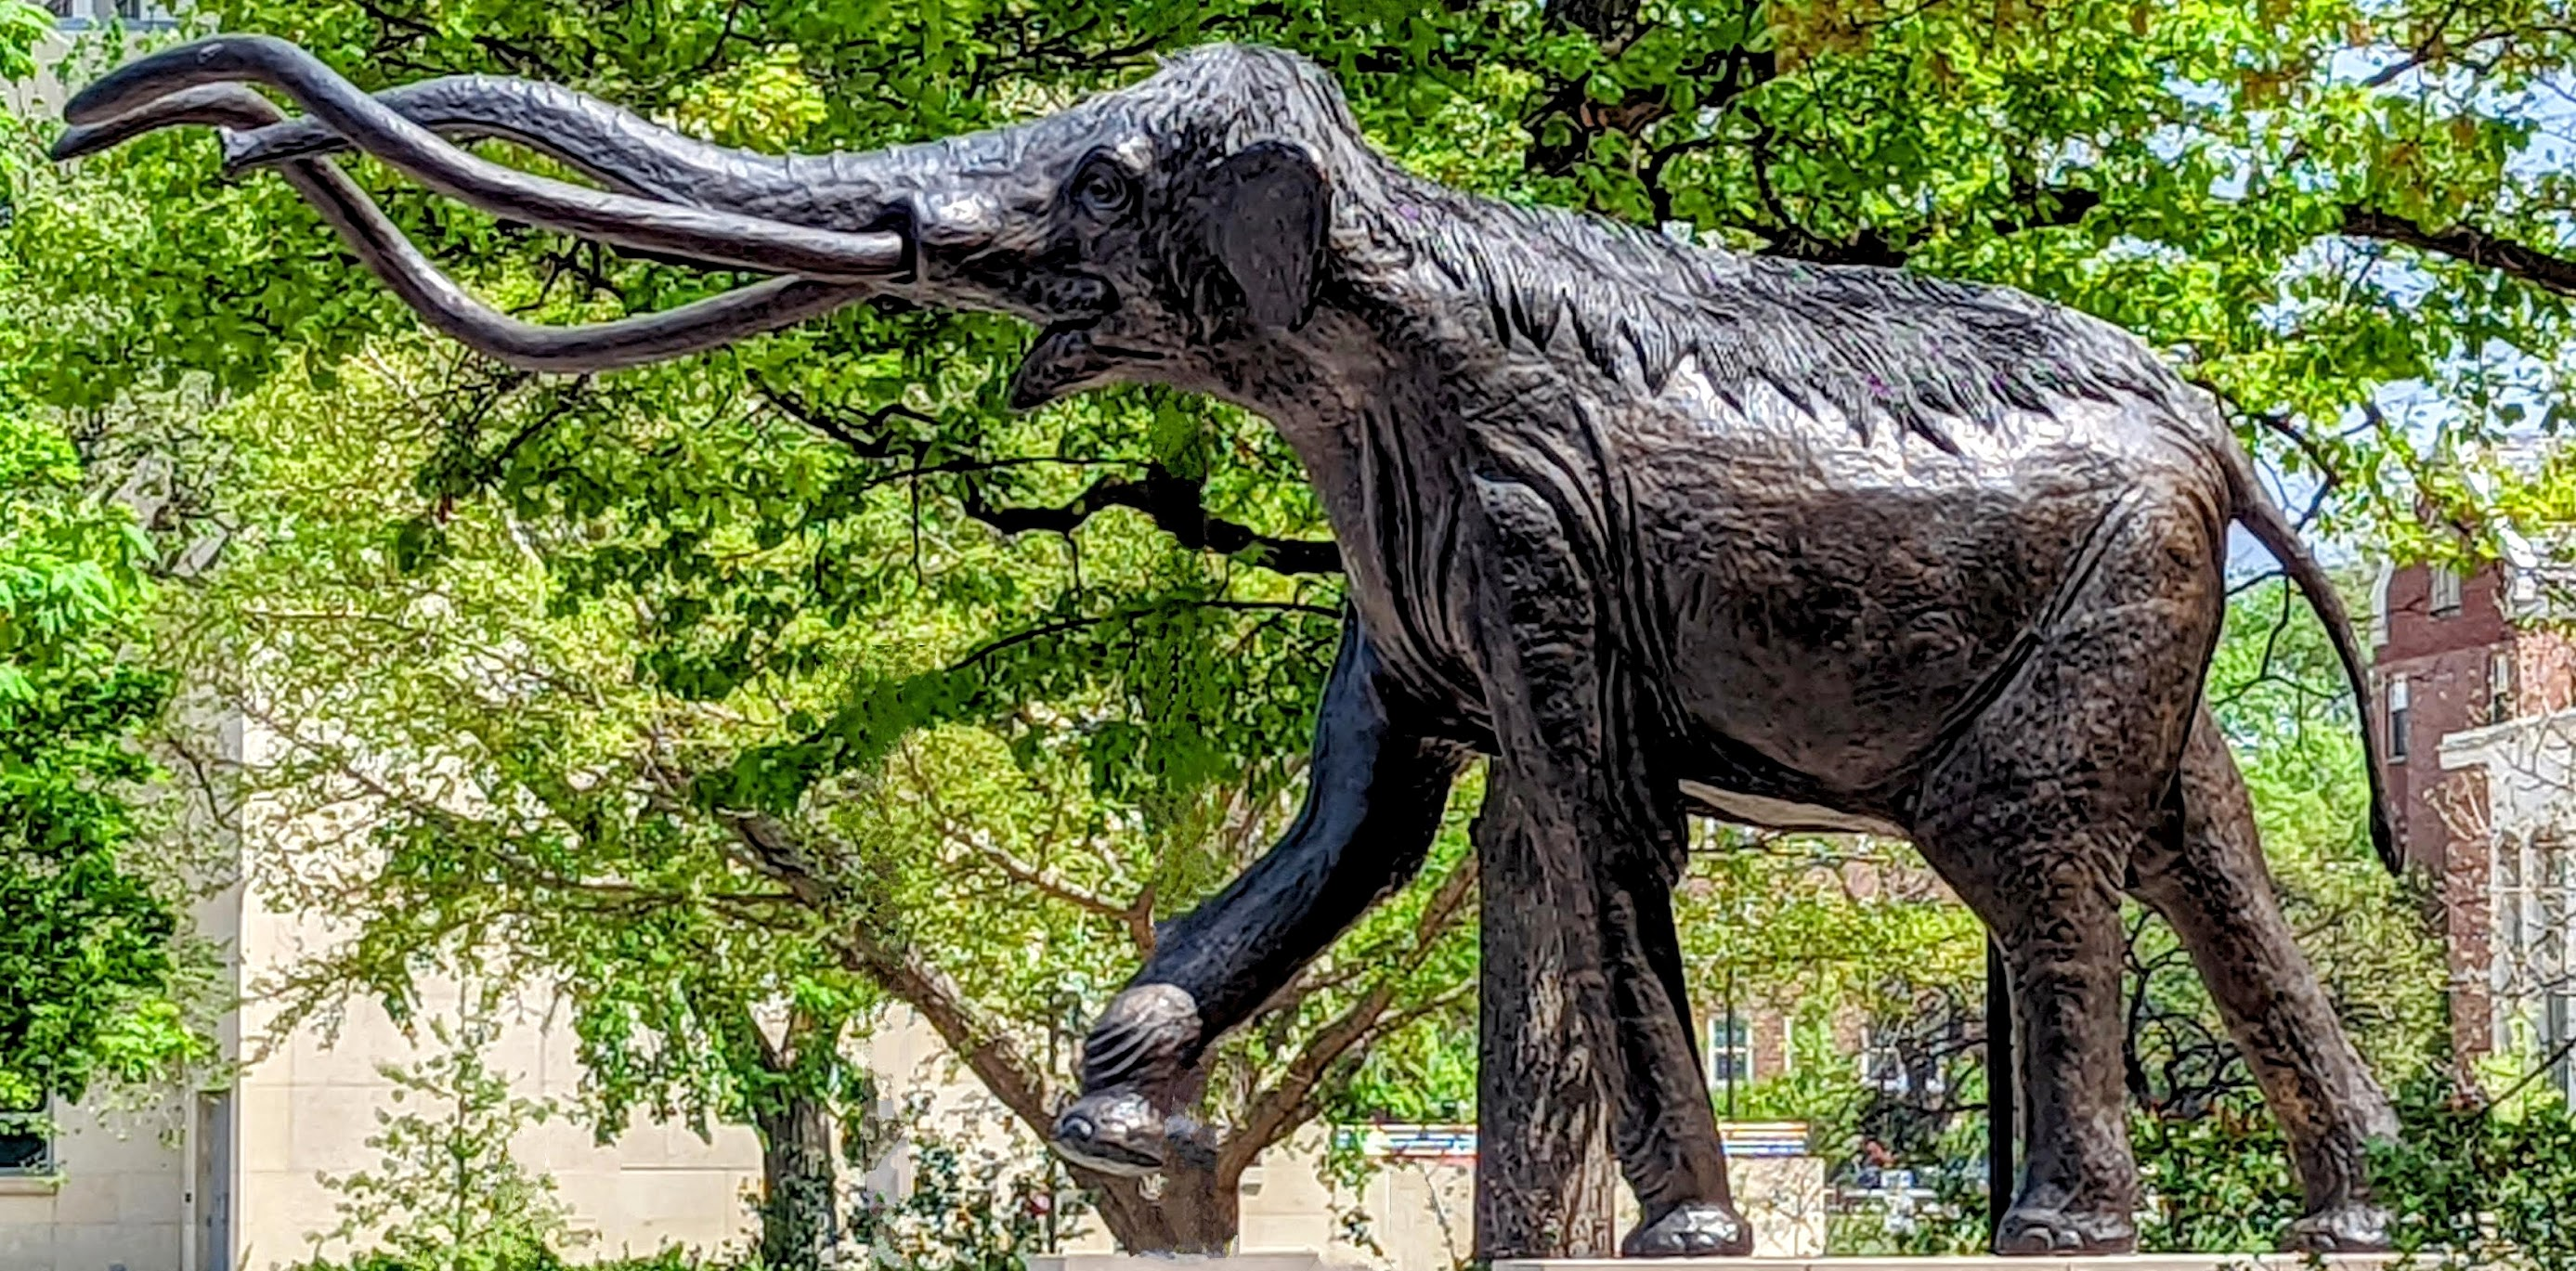
\includegraphics[width=.4\textwidth]{archie}
        \caption{Archie.\\ \footnotesize{Photograph by Bohn.}}
    \end{wrapfigure}

    You're relaxing at your favorite hangout when another customer catches your attention.
    He's rather large (dare I say, \textit{mammoth}), a bit hairy, and looking frustrated in front of his laptop.
    ``I'm Archie,'' he says, ``and I'm trying to teach myself this card game called \textit{Poker}.
    I found this source code that I thought I could use to understand Poker better, but the code is incomplete, and I don't entirely understand what's there.
    Could you explain the code to me, please?'
}

\newcommand{\GetHired}{
    Archie's face lights up in a very big smile.
    ``Thanks!''
    After pausing in thought for a moment, he says, ``Say, I've got a new startup company that could really use your help.
    Are you interested?
    It'll be exciting!''
}

\newcommand{\FirstDayOnTheJob}{
    \begin{wrapfigure}{r}{0.33\textwidth}
        \centering
        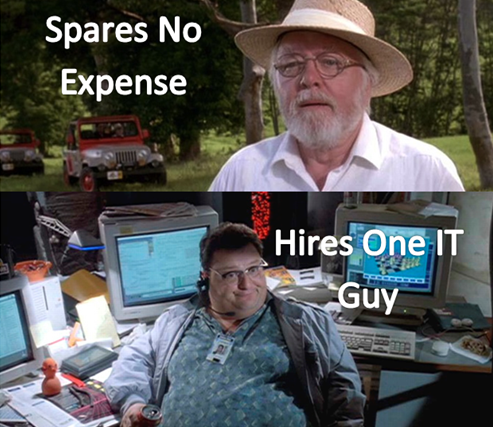
\includegraphics[width=.4\textwidth]{some-expenses-spared}
        \caption{Some expenses were spared.\\ \footnotesize{Original images \textcopyright\ Universal Studios and Amblin Entertainment, Inc. Meme creator unknown.}}
    \end{wrapfigure}

    You've recently been hired to help get the Pleistocene Petting Zoo get started.
    Your new employer, Archie, is surprisingly honest: he admits to you that some expenses were spared.
    Archie cheerfully points out that any challenge is also an opportunity to succeed.
    You suspect your job will offer plenty of ``opportunities to succeed.''
}

\newcommand{\HasKeyboard}{
    Great news!
    Archie brings you your new keyboard.
    He also brings you a problem of his own.
    Because you were held up with the broken keyboard, Archie decided to try some programming on his own, and his code is behaving strangely.
}

\newcommand{\ArchieWroteSmellyCode}{
    Working at the Pleistocene Petting Zoo certainly is proving to be interesting.
    You're glad that you don't have to worry about the problem of the giant sloths very slowly chasing their handlers, but now it seems that Archie has decided to try to write a program or two.
    At a glance, his code is smellier than the wooly rhinoceros' enclosure.
    But you take a closer look anyway to try to understand why his code acts strangely.
}

\newcommand{\InsurancePreview}{
    You hear somebody enter the room.
    ``\textit{Frankenstein}, `boat','' is the challenge, and she answers, ``borne.''
    Archie introduces you to the new arrival, ``Lil, this is our new developer, the one who wrote the app we just used.''
    He turns to you: ``This is Lilith Redd from business operations.''
    He turns back to her and continues, ``Lil, what's the good word?''

    ``The word isn't good, I'm afraid.
    I just heard back from the insurance company.''
}

\newcommand{\OnLoanToEclecticElectronics}{
    All work at the Pleistocene Petting Zoo has stopped while Archie tries to find a $\cancelto{\mathrm{reasonable}}{\mathrm{gullible}}$ insurance company.
    Rather than furloughing staff, he's asked everybody to help out with his other startup companies for a week or two.
    He specifically asked that you help out with Eclectic Electronics.

    Herb Bee, the chief engineer, explains that Eclectic Electronics is developing a patent-pending C-licon tool that will convert C code into an integrated circuit that has the same functionality as the original C code.
    To test it out, he tasked you with writing the code to implement an Arithmetic Logic Unit (ALU).
    Your task will be to implement integer addition, subtraction, multiplication, and division.
    Even though high-level languages' \textit{logical} boolean operations normally are not part of an ALU, Herb wants you to include these in the ALU to see if that can make some programs run faster.
    Because bitwise operations and bit shift operations have been implemented, you will be able to use C's bitwise and bit shift operators, but because arithmetic operations have not yet been implemented, you cannot use C's arithmetic operators.
    Because C library functions generally make use of arithmetic operations (which have not yet been implemented), you cannot use library functions.
}

\newcommand{\SuccessfulALU}{
    Herb smiles as he hands you the the test results from the latest integrated circuit fab batch.
    ``C-licon successfully turned your code into an ALU.
    Nicely done!''
    I think maybe it's time to use C-licon to see if we can improve the Floating Point Unit (FPU) on our experimental microprocessor.
}

\newcommand{\WriteAnFPU}{
    Herb tells you that, Eclectic Electronics tested the integrated circuit that the C-licon tool created from your ALU code, and they've concluded that C-licon is ready to use for their new experimental microprocessor.
    He tasks you with writing C code (that will be used by the C-licon tool) to implement a Floating Point Unit (FPU).
    Your task will be to implement floating point addition, subtraction, multiplication, and division.
    You can use any bit operations and, thanks to the ALU you wrote, you can use any integer arithmetic operations (use the conventional + - * / operators).
    Because the FPU has not yet been implemented, you cannot use C's floating point operations, you cannot use \lstinline{float}s nor \lstinline{double}s, and you cannot use library functions.
}

\newcommand{\GoingBackToTheZoo}{
    Lil enters the room.
    Herb challenges her: ``\textit{Gulliver's Travels}, `endian','' and Lil answers, ``ends.''

    Lil walks up to you and says, ``We have the insurance situation taken care of, and it's time to get the Zoo ready for guests.
    We're reassembling the tech team, and there's plenty of work to do.''

    You smile.
    ``That's good news!''

    Lil's face is hard to read.
    ``Well, yes and no.
    It's good that you'll be able to resume work on the Zoo's systems.
    But while Archie was waiting for us to fix the insurance situation, he got bored and -- cutting a long story short -- he ended up creating some new `opportunities' that we need you `to succeed' at.''
}

\newcommand{\SettledIntoRoutine}{
    You've settled into a comfortable routine at the Pleistocene Petting Zoo.
    While your job isn't quite as exciting as that of the saber-toothed tigers' dentist, it still has something new and interesting almost every day.

    Archie announces that he heard that hand-crafted assembly code can be faster than high-level language code.
    You try to explain that while this may have been true decades ago, modern optimizing compilers generate code faster than what a typical programmer can achieve with assembly code.
    Archie doesn't believe you and insists that you write the zoo's new cipher program in x86 assembly code.
}

\newcommand{\NewmanRanOffWithSamples}{
    Archie is hurriedly packing is trunk, like he's about to leave on a short-notice urgent trip.
    Before charging out the door, he pauses to tell you, ``Newman just stole some of our samples.
    I need to track him down before he sells them to the Supersized Safari Syndicate.
    I guess this means you're in charge of the Zoo's computer system now.
    Don't worry, you'll be fine. What could possibly go wrong?''
}

\newcommand{\BombLabIntroduction}{  % Ties Bryant & O'Halloran's Bomb Lab into the Pleistocene Petting Zoo story
    In a jarring collision of movie franchises, the CEO of Virtucon makes a Zoom call to the Pleistocene Petting Zoo.
    For some reason that nobody really explains, you're the only person available to handle the situation.
    The guy, who sounds kind of like an animated ogre, demands that the Pleistocene Petting Zoo deliver to him a megalodon shark with a head-mounted laser capable of emitting a beam of pure antimatter.

    You blurt out, ``Then it's not a laser,'' and then try to explain to him that megalodons are from the Miocene epoch, and expecting to find them at the Pleistocene Petting Zoo would be as ridiculous as a Cretaceous-period tyrannosaur at a Jurassic-themed park.

    ``Zip it!'' commands the guy who kind of looks like the host of a public-access show you used to watch.
    ``Since you won't meet my demand, my minions have placed a `binary bomb' under your zoo.
    Because I like really convoluted plans, we put software on your Linux server that controls the bomb.
    If you do nothing, the bomb will explode.
    If you turn off the Linux server, the bomb will explode.
    If you go slower than 50mph, the bomb will -- no, never mind that last part.

    ``The bomb software consists of a sequence of phases.
    Each phase expects you to type a particular string on \texttt{stdin}.
    If you type the correct string, then the phase is {\em defused} and the bomb proceeds to the next phase. Otherwise, the bomb {\em explodes}.
    The bomb is defused when every phase has been defused.

    ``Your mission, which you have no choice but to accept, is to defuse your bomb before the due date.
    Good luck, and welcome to the bomb squad!''
}

\newcommand{\FoodLockersAreStuck}{
    Having saved the Zoo from Dr. Evil's binary bomb, you relax back in your chair and think about taking a break.
%SPRINGBREAK
    Maybe an entire week in which you don't have solve any problems or meet any deadlines -- that'd be real nice.
%FALLBREAK
    % Maybe 4-day weekend in which you don't have solve any problems or meet any deadlines -- that'd be real nice.

    Another Zoom call comes in.
    \textit{What now!?} you wonder as you take your feet off of the desk to answer the call.
    An uncomfortable-looking animal handler says, ``We can't unlock the food lockers.
    It's the animals' feeding time, and we can't open the food lockers!
    It's feeding time, we can't get to the animals' food, and,'' his eyes dart nervously toward the animal enclosures, ``and many of them have sharp, pointy claws and others have big, stompy feet.''
}

\newcommand{\AttackLabIntroduction}{    % Ties Bryant & O'Halloran's Attack Lab into the Pleistocene Petting Zoo story
    You managed to keep the Pleistocene Petting Zoo from blowing to smithereens, but it turns out that Dr. Evil's minions weren't too careful when they put the bomb control software on the Zoo's Linux server.
    The software that controls the food locker has been heavily damaged!
    The functions that unlock the food locker doors are still present, but there's no way to activate those functions.

    You then recall what Archie told you when he hired you: some expenses were spared.
    You run the machine code through a disassembler and quickly see that it has a buffer overflow vulnerability.
    Before the situation in the dire wolf enclosure gets too dire, you sit down and get to work.

    The \function{ctarget} code runs on an older machine that allows executable code to be present on the stack, so it's vulnerable to a conventional code injection buffer overflow attack.
    \begin{itemize}
        \item Phase 1 (\function{touch1}) unlocks the food locker so the animal handlers can prepare the food.
        \item Phase 2 (\function{touch2}) opens the doors between the food locker and the carnivore enclosures;
        you will need to pass a cookie to the function to authenticate yourself.
        \item Phase 3 (\function{touch3}) closes the doors between the food locker and the carnivore enclosures.
    \end{itemize}
    The \function{rtarget} code runs on a newer machine that does not allow executable code to be present on the stack, so you'll have to conduct a return-oriented programming attack on it.
    \begin{itemize}
        \item Phase 4 (\function{touch2)} opens the doors between the food locker and the herbivore enclosures;
        you will need to pass a cookie to the function to authenticate yourself.
        \item Phase 5 (\function{touch3}) closes the doors between the food locker and the herbivore enclosures.
    \end{itemize}
}

\newcommand{\MostAnimalsAreFed}{
    Before you take on the Phase 5, pause to consider what you have accomplished so far.
    In Phases 2 and 3, you caused a program to execute machine code of your own design.
    If {\sc ctarget} had been a network server, you could have injected your own code into a distant machine.
    In Phase 4, you circumvented two of the main devices modern systems use to thwart buffer overflow attacks.
    Although you did not inject your own code, you were able inject a type of program that operates by stitching together sequences of existing code.
    Also, all animals have been fed, the carnivores are still in their enclosure, the mammoths can't fit through the herbivore door, and only the giant sloths seem interested in very slowly escaping.
}

\newcommand{\ArchieReturns}{
    Archie returns from tracking down Newman, who'd run off with some of the Pleistocene Petting Zoo's samples shortly before Dr.~Evil's Zoom call.
    ``It turns out he didn't get very far at all,'' Archie sighs.
    ``He ran into a flock of terror birds as he was leaving, and we found him in one of the emergency shelters.

    Archie smiles. ``I trust things were uneventful while I was away?''
}

\newcommand{\PickingUpNewmansProject}{
    Archie seems genuinely surprised that Newman is refusing to go back to work.
    ``You would think that he'd be grateful for being rescued from that flock of terror birds.''
    Before you can wonder out-loud whether it would be a good idea to trust someone who had just tried to sell trade secrets to a competitor, Archie gives you your new task.

    ``Because Newman isn't cooperating, I need you to finish the project he was working on.
    As you can imagine, duplicating the genetic information for our exhibits can take a long time, and Newman realized that we might be able to duplicate the data faster if we had a concurrent program which has one thread reading from the original data and another thread writing the copy.
    Unfortunately, he ran off to sell samples to the  Supersized Safari Syndicate before finishing the duplicator.
    Right now the duplicator seems to work, but it usually makes imperfect copies.
    Have you ever seen a paleolama with two noses, four eyes, and no ears!?''
}

\newcommand{\WeNeedBetterDetection}{
    Between Newman trying to sell samples to a competitor, that weird guy almost blowing up the zoo, and the animals almost escaping, Archie is getting worried.
    ``I think we need to introduce additional protective measures.
    As useful as your challenge-response app is in helping us detect intruders, I think it's now clear that we need something that will detect someone -- or some\textit{thing} -- when they're someplace they shouldn't be, even when no one else is around.
    I've asked the team at Eclectic Electronics to put something together.''
}

\newcommand{\WeNeedBetterLocks}{
    Between Newman trying to sell samples to a competitor, that weird guy almost blowing up the zoo, and the animals almost escaping, Archie is getting worried.
    ``I think we need to introduce additional protective measures.
    As useful as your challenge-response app is in helping us detect intruders, I think it's now clear that we need something that will keep someone -- or some\textit{thing} -- out of places they shouldn't be, even when no one else is around.
    I've asked the team at Eclectic Electronics to put something together.''
}

\newcommand{\IntroduceHardware}{
    Archie walks up to you, along with Herb Bee from Eclectic Electronics.
    Herb is holding a tangled mess of electronics.
    Archie explains, ``Herb here has developed a prototype of a device that he thinks will be useful for our physical security needs, as well as a few other applications around here. He calls it the \textit{Cow Pi}.''

% TODO: parameterize based on which microcontroller is actually being used
    You look at the device in Herb's hands and see the \nano\ central to the circuit.
    ``Isn't \textit{-Pi} typically used as a suffix for circuits that use a Raspberry Pi instead of an Arduino?''

    Herb replies, ``Typically, yes, but \textit{Cowduino} isn't very punny, is it?''

    Archie chimes in, ``Maybe with the right emphasis: \textit{Cow-DOO-ino}.''

    ``That's kind of subtle, don't you think? How will people know to put the emPHAsis on that sylLAble?''

    ``I think we're getting off topic here,'' you point out.
    ``How can I help?''

    ``Oh, right,'' Herb says, ``We'd like you to kick its proverbial tires.
    Let's start off with something simple, like a number builder tool.''
}

\newcommand{\JeffGoldblum}{
    Herb looks over your work.
    ``Hmm, yes. I think this is coming along nicely.
    Let's run a few more tests.''

    Archie storms into the room.
    ``We have \textit{got} to do something about security!
    How's that doodad coming along?
    Because there's now a half-man/half-fly in the labs going on-and-on about Chaos Theory and how if we just give him a MacBook and a spaceship then he'll be able to get the Lord of Thunder to travel across the 8th Dimension.
    Is that thing just about ready?''

    Herb shakes his head, ``No, not quite yet. It should be ready in about a week.''
}

\newcommand{\DisdainfulHerb}{
    Smoke wafts from Herb's soldering iron as he looks up when you approach.
    Cleaning the iron's tip, he quotes:
    ``Somebody once said, `The three most dangerous things in the world are a programmer with a soldering iron, a hardware engineer with a software patch, and'{}'' -- he glances nervously in Archie's direction -- ``{}`a user with an idea.'\footnote{
        Rick Cook, \textit{The Wizardry Consulted}, 1995.
    }$^{\mathrm{,}}$\footnote{
        The notion of being wary of programmers wielding screwdrivers or soldering irons long pre-dated this quote, as there are apocryphal tales of people who found it easier to modify the hardware to suit the software rather than the other way around.
    }''
}

\newcommand{\NumberConversionTool}{     % Since we're now allowing `sprintf()` with the LCD1602, converting between decimal and hexadecimal is trivial; it still might be okay for 7-segment displays
    Herb gets straight to the point.
    ``We promised Archie that we'd be able to start using the Cow Pi to build systems in a week.
    So far we've tested its input/output functionality, but we still need to test its timer and also whether we can take inputs without constantly polling the input devices.
    As before, we don't need to do anything too fancy;
    let's try a number base conversion tool.''
}

\newcommand{\LessDisdainfulHerb}{
    Smoke wafts from Herb's soldering iron as he looks up when you approach.
    Cleaning the iron's tip, he notes:
    ``Somebody once said that one of the most dangerous things in the world is a programmer with a soldering iron.''\footnote{
        ``The three most dangerous things in the world are a programmer with a soldering iron, a hardware engineer with a software patch, and a user with an idea.'' -- Rick Cook, \textit{The Wizardry Consulted}, 1995.
    }$^{\mathrm{,}}$\footnote{
        The notion of being wary of programmers wielding screwdrivers or soldering irons long pre-dated this quote, as there are apocryphal tales of people who found it easier to modify the hardware to suit the software rather than the other way around.
    }
}

\newcommand{\RemoteControlledCar}{

    About this time, Archie walks by, thinking about electric carts to transport visitors around the Pleistocene Petting Zoo.
    ``They probably should be remote-controlled.''
    He looks at you and Herb, and asks, ``Do you think you could make a cart a remote-controlled cart?''

    You ask the obvious question, ``Are there carts here already?''

    Archie waves his hand in the air, dismissing that detail, ``Not yet, but could you make the remote-control?''
    
    You hestatingly summarize: ``You want a cartless remote-controlled cart?''

    Archie beamingly smiles, ``Exactly!''

    Herb jumps in, ``Yes, we'll do it.''
    Herb looks at you and adds, ``It'll give us a chance to test the Cow Pi's timer and whether we can take inputs without constantly polling the input devices.''
}

\newcommand{\LauraDern}{
    You and Herb look for Archie in the Pleistocene Petting Zoo's labs to give him the good news, and you find a blond woman wearing cargo shorts, butchering a Gilbert and Sullivan song\dots \\ \\
    \textmusicalnote\ I am the very model of a modern vice admiral \textmusicalnote \\
    \textmusicalnote\ I've information about all things paleobotanical \textmusicalnote \\
    \textmusicalnote\ And I've been up to my armpits in problems scatological \textmusicalnote \\
    \textmusicalnote\ During the regency I had experience matriarchical \textmusicalnote \\
    \textmusicalnote\ I plot space travel, normal and superluminal \textmusicalnote \\
    \textmusicalnote\ (Even if I challenge the Pauli exclusion principle) \textmusicalnote \\

    ``I don't know how these people keep getting into our labs.
    \textit{Please} tell me that you have good news,'' pleads Archie.

    ``Yes, the Cow Pi is ready for whatever you need: calculators, security systems, parking meters -- you name it,'' Herb cheerfully responds.

    ``Excellent.''
    Archie turns to you.
    ``I'd like you and Newm... no, \textit{not} Newman.
    I'd like you and someone else on the staff to get started right away.
    Here's what I'd like to have built first.''
}

\newcommand{\CalculatorNeeded}{
    ``I have various teams working on different projects around here to improve security,'' Archie reminds you.
    He glances toward the Zoo's labs, where there's now a guy who looks like the actor who portrayed the fictional actor who portrayed the Norse god Odin, trying to avoid children while wistfully talking about raising rabbits in Montana.
    You briefly wonder why there are children someplace where there are also carnivorous megafauna, and then you remember that you work at a petting zoo.
    ``What I need your team to do,'' Archie continues, ``is make a four-function calculator so that we can quickly and easily determine whether we have the correct number of specimens, or if any are missing.''
}

\newcommand{\CalculatorCounting}{
    Technicians are using your calculator to compute how many specimens are still present in the lab, and establish that all specimens are accounted for after Newman's attempted theft.
    As reports come in of facilities getting secured with Cow Pi-based locks and passages being monitored with Cow Pi-based motion sensors, Archie smiles and tells you that this was a job well done.
    With all of the excitement neatly wrapped-up and arriving at a satisfactory conclusion, you look forward to a boring career in which there's absolutely no screaming and running for your life.
}

\newcommand{\CombinationLockNeeded}{
    ``I have various teams working on different projects around here to improve security,'' Archie reminds you.
    He glances toward the Zoo's labs, where there's now a guy who looks like the actor who portrayed the fictional actor who portrayed the Norse god Odin, trying to avoid children while wistfully talking about raising rabbits in Montana.
    You briefly wonder why there are children someplace where there are also carnivorous megafauna, and then you remember that you work at a petting zoo.
    ``What I need your team to do,'' Archie continues, ``is make a combination lock so that only authorized people can get into our lab facilities.''
}

\newcommand{\CombinationLockInstalled}{
    After fastening the new electronic combination lock to the lab door, Archie smiles and tells you that this was a job well done.
    With all of the excitement neatly wrapped-up and arriving at a satisfactory conclusion, you look forward to a boring career in which there's absolutely no screaming and running for your life.
}

\newcommand{\RangeFinderNeeded}{
    ``I have various teams working on different projects around here to improve security,'' Archie reminds you.
    He glances toward the Zoo's labs, where there's now a guy who looks like the actor who portrayed the fictional actor who portrayed the Norse god Odin, trying to avoid children while wistfully talking about raising rabbits in Montana.
    You briefly wonder why there are children someplace where there are also carnivorous megafauna, and then you remember that you work at a petting zoo.
    ``What I need your team to do,'' Archie continues, ``is make a range finder that will alert us when someone -- or some\textit{thing} -- gets too close to someplace they shouldn't be.''
}

\newcommand{\RangeFinderDetecting} {
    A technician installing a new range finder outside the lab door briefly sets off the alarm, but then the range finder falls quiet and faithfully reports that nothing is approaching.
    As reports come in of facilities getting secured with Cow Pi-based locks, and of accurate speciment counts accomplished with Cow Pi-based calculators, Archie smiles and tells you that this was a job well done.
    With all of the excitement neatly wrapped-up and arriving at a satisfactory conclusion, you look forward to a boring career in which there's absolutely no screaming and running for your life.
}

\usepackage{amsmath}
%\usepackage{array,color,colortbl}
\definecolor{LightGreen}{rgb}{0.88,1,0.88}
\usepackage{multicol}
\usepackage{CJKutf8}
\usepackage{gensymb}
\usepackage{graphicx}
\usepackage{multirow}
\setlength{\columnsep}{2cm}
\newcommand{\power}{power~({\color{red}\textbf{+}}) rail}
\newcommand{\ground}{ground~({\color{blue}\textbf{--}}) rail}



% \captionsetup{width=.8\linewidth}

% \lstset{language=c, numbers=left, showstringspaces=false,
%     moredelim = [s][\ttfamily]{/*}{*/} % I shouldn't need this parameter!
%     }

\renewcommand{\labnumber}{\capstonelabnumber}
\renewcommand{\labname}{Implementing a Range Finder and Alarm}
\renewcommand{\shortlabname}{rangefinder -- grouplab}
\renewcommand{\collaborationrules}{\capstonelabcollaboration}
\renewcommand{\duedate}{\capstonelabdue}
\newcommand{\nano}{\developmentboard} % TODO: replace \nano with \developmentboard
\renewcommand{\runtimeenvironment}{\capstonelabenvironment}
\pagelayout
\begin{document}
    \labidentifier

    \pdfbookmark[1]{Frontmatter}{frontmatter}                           In this assignment, you will write code for \runtimeenvironment\ that will use new electronic devices to interact with the physical world.

The instructions are written assuming you will edit the code in the Arduino IDE and run it on \runtimeenvironment, constructed according to the pre-lab instructions.
If you wish, you may edit the code in a different environment; however, our ability to provide support for problems with other IDEs is limited.

\section*{Learning Objectives}

After successful completion of this assignment, students will be able to:
\begin{itemize}
    \item Work collaboratively on a hardware/software project
    \item Design and implement a simple embedded system
    \item Expand their programming knowledge by consulting documentation
\end{itemize}

\subsection*{Continuing Forward}

This penultimate lab assignment does not contribute to the final lab assignment.
By integrating elements of what you learned in this course, and by demonstrating that you can review documentation to learn on your own, to design a small embedded system, you will show how much progress you have made this semester.

\section*{During Lab Time}

During your lab period, coordinate with your group partner(s) to decide on your working arrangements.
Unless you're only going to work on the assignment when you're together, you may want to set up a private Git repository that is shared with your partner(s).
With your partner(s), modify your hardware kit as described in Section~\ref{sec:hardwareMods}.
Then, think through your system's design and begin implementing it.
The TAs will be available for questions.


    \softwareengineeringfrontmatter

    \section*{Scenario}                                                 \RangeFinderNeeded

    \section{Assignment Summary}                                        This assignment is principally about getting comfortable when explicitly working with memory.
Being able to think about a value and a reference to that value distinctly will improve your programming skills in any language.

Before you do so, in Section~\ref{sec:archiesCode} you will examine Archie's code.
Parts of Archie's programs use code that the C standard explicitly states will result in undefined behavior.
By understanding the mistakes that Archie made, we hope that you can avoid them in your own code.

In Section~\ref{sec:challengeResponse}, you will build and use a linked list.
This will require you to allocate space for the list's nodes and manipulate pointers that connect the nodes to each other.

\ifboolexpe{not bool{allowspaghetticode}}{
    There are no particular restrictions in this assignment other than those common to most lab assignments in this course.
    You can check whether you're using a \lstinline{goto} or \lstinline{continue} statement, or whether you're using \lstinline{break} or \lstinline{return} to exit a loop, by running the constraint-checking Python script:
    \texttt{python constraint-check.py linkedlistlab.json}
}{}


    \section{Getting Started} \label{sec:GettingStarted}                Download \textit{\shortlabname.zip} or \textit{\shortlabname.tar} from \filesource\ and copy it to \runtimeenvironment.
Once copied, unpackage the file.
Four of the five files (\textit{alu.h}, \textit{basetwo.c}, \textit{alu.c}, and \textit{integerlab.c}) contain the starter code for this assignment.
The last file (\textit{Makefile}) tells the \texttt{make} utility how to compile the code.
To compile the program, type:

\texttt{make}

This will produce an executable file called \textit{integerlab}.

When you run the program with the command \texttt{\textbf{\textit{./integerlab}}}, you will be prompted:

\begin{verbatim}
    Enter a one- or two-operand logical expression,
        a two-operand comparison expression, a two-operand arithmetic expression,
        "lg <value>" or "exponentiate <value>" to test your powers-of-two code,
        "is_negative <value>" to determine if 2's complement value is negative,
        "add1 <binary_value1> <binary_value2> <carry_in>" for 1-bit full adder,
        "add32 <hex_value1> <hex_value2> <carry_in>" for 32-bit ripple-carry adder,
        or "quit":
\end{verbatim}

When you enter a value, if it is prepended with \texttt{\textbf{\textit{0x}}} then the parser will parse it as a hexadecimal value;
otherwise, except as noted in Sections~\ref{subsec:one-bit-full-adder} and \ref{subsec:ripple-carry-adder}, the parser will treat it as a decimal value.

For now, type \texttt{\textbf{\textit{quit}}} to exit the program.

\subsection{Description of IntegerLab Files}

\subsubsection{integerlab.c}

Do not edit \textit{integerlab.c}.

This file contains the driver code for the lab.
It parses your input, calls the appropriate arithmetic function, and displays the output.

\subsubsection{alu.h} \label{subsubsec:alu.h}

Do not edit \textit{alu.h}.

This header file contains two type definitions:
\begin{description}
    \item[one\_bit\_adder\_t] is a structure to hold the 1-bin inputs (\lstinline{a}, \lstinline{b}, \lstinline{c_in}) and 1-bit outputs (\lstinline{sum}, \lstinline{c_out}) of a one-bit full adder.
    \item[alu\_result\_t] is a structure to hold the outputs from an arithmetic logic unit.
        Its fields are:
        \begin{itemize}
            \item \lstinline{result}, a 16-bit bit vector that is considered ``the'' result of the computation
            \item \lstinline{supplemental_result}, a 16-bit bit vector that stores additional result data from instructions that place their results in two registers
            \item \lstinline{unsigned_overflow}, a 1-bit flag to indicate whether overflow occurred when interpreting the source operands as unsigned values
            \item \lstinline{signed_overflow}, a 1-bit flag to indicate whether overflow occurred when interpreting the source operands as signed values
            \item \lstinline{divide_by_zero}, a 1-bit flag to indicate whether there was an attempt to divide by zero.
        \end{itemize}
\end{description}

The header file also contains two macros, \function{is_zero()} and \function{is_not_zero()} to bootstrap your ALU code.
These macros act like functions and return a boolean value to indicate whether an integer is 0 or not.\footnote{
    The astute student will quickly realize that \function{is_not_zero()} is not necessary and, with a little thought, will realize that they can \function{is_zero()} as a function within the constraints of this assignment.}

The header file also contains several function declarations.
The requirements for these functions will be discussed later in this assignment.

\subsubsection{basetwo.c}

This is the first of two files that you will edit.

There are two functions in \textit{basetwo.c} that will allow you to demonstrate an understanding of powers-of-two and/or an understanding of some uses of bit shifts.
\begin{description}
    \item[lg()] returns the base-2 logarithm of its argument, assuming its argument is a positive power-of-two;
        if the argument is 0 or is not a power-of-two, then there are no guarantees about the function's return value
    \item[exponentiate()] creates a power-of-two by raising 2 to the provided exponent, assuming the exponent is a non-negative value strictly less than 32;
        if the argument is negative or is greater than 31, then there are no guarantees about the function's return value
\end{description}
These functions are inverses of each other: $x = \log_2 2^x$, and $y = 2^{\log_2 y}$.

Strictly speaking, you can write your ALU code without these functions;
however, some students in the past had difficulty finding solutions for their ALU code without obtaining a base-2 logarithm and/or calling a function to create a power-of-two.
Rather than tempt you to violate one of the assignment's constraints by calling the \textit{math} library's \function{log2()}, \function{exp2()}, and/or \function{pow()} functions, we now have you write your own code for these functions.

\subsubsection{alu.c}

This file will contain most of the code that you write, and the functions in \textit{alu.c} are in the order in which you will likely write them.
\begin{itemize}
    \item A simple check
        \begin{description}
            \item[is\_negative()] returns a boolean value to indicate whether the argument, when interpreted as a signed integer, is negative
        \end{description}
    \item Equality comparisons
        \begin{description}
            \item[equal()] returns \lstinline{true} if and only if $value1 = value2$
            \item[not\_equal()] returns \lstinline{true} if and only if $value1 \not = value2$
        \end{description}
    \item Logical operations
        \begin{description}
            \item[logical\_not()] returns the logical inverse of the argument
            \item[logical\_and()] returns the logical conjunction of the two arguments
            \item[logical\_or()] returns the logical disjunction of the two arguments
        \end{description}
    \item Addition and subtraction
        \begin{description}
            \item[one\_bit\_full\_addition()] performs addition for one bit position, determining both the sum bit and the carry-out bit
            \item[ripple\_carry\_addition()] adds two 32-bit values to each other and to a carry-in bit
            \item[add()] adds two 16-bit values to each other
            \item[subtract()] subtracts a 16-bit value from another
        \end{description}
    \item Inequality comparisons
        \begin{description}
            \item[less\_than()] returns \lstinline{true} if and only if $value1 < value2$
            \item[at\_most()] returns \lstinline{true} if and only if $value1 \leq value2$
            \item[at\_least()] returns \lstinline{true} if and only if $value1 \geq value2$
            \item[greater\_than()] returns \lstinline{true} if and only if $value1 > value2$
        \end{description}
    \item Unsigned multiplication and division
        \begin{description}
            \item[multiply\_by\_power\_of\_two()] multiplies the first argument by the second, assuming that the second argument is zero or a power of two;
                there are no guarantees if this assumption is not satisfied
            \item[unsigned\_multiply()] multiplies two 16-bit values to each other, if the arguments are interpreted as unsigned integers
            \item[unsigned\_divide()] divides a 16-bit value by another, if the arguments are interpreted as unsigned integers
        \end{description}
    \item Signed multiplication and division (bonus credit)
    \begin{description}
        \item[signed\_multiply()] multiplies two 16-bit values to each other, if the arguments are interpreted as signed integers
        \item[signed\_divide()] divides a 16-bit value by another, if the arguments are interpreted as signed integers
    \end{description}
\end{itemize}


    \section{Modifying the Hardware Circuit} \label{sec:hardwareMods}   You will need to make some changes to your Cow Pi circuit before you can start this lab.

\subsection{Necessary Components}

Figure~\ref{fig:components} shows the components you will need for the range finder and alarm.

\begin{figure}
    \centering
    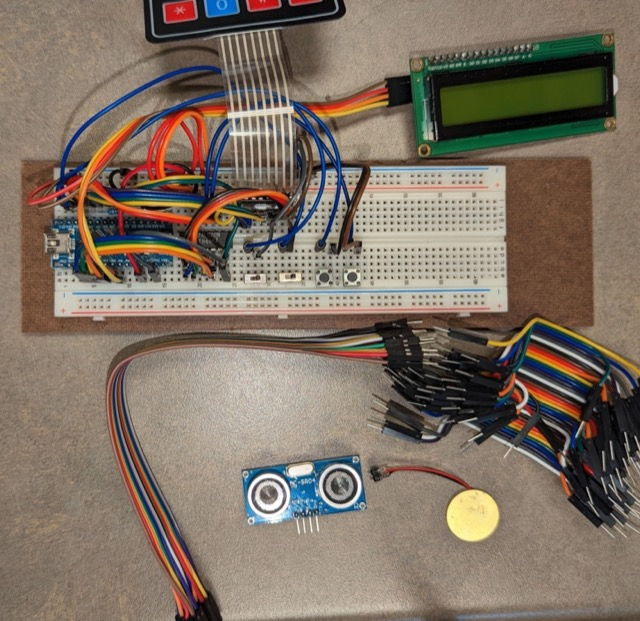
\includegraphics[width=10cm]{reconfiguration_images/components}
    \caption{Components needed for the Range Finder \label{fig:components}}
\end{figure}

You will need:
\begin{itemize}
    \item Your Cow Pi hardware circuit
    \item A piezoelectric disc
        \begin{itemize}
            \item Piezoelectric devices can convert electric energy into mechanical energy, and vice-versa
            \item You will use a piezoelectric disc to create an audible alarm
        \end{itemize}
    \item An ultrasonic echo sensor
        \begin{itemize}
            \item The two prominent drums on this device are ultrasonic transducers, one of which converts electricity to 40kHz sound (well above the range of human hearing), and the other of which converts 40kHz sound into electricity
            \item You will measure the time between the ultrasound being transmitted and its reflecting being received to determine the distance to whatever is reflecting the ultrasound
        \end{itemize}
    \item Two 20cm male-to-male wires and (optionally) two additional male-to-male wires
\end{itemize}

You and your partner only need to modify one of your Cow Pis (but you may modify both).

\subsection{Connecting the Piezoelectric Disc}

The \developmentboard's pin D9 is currently used for the right pushbutton.
In the group project, we will use it to control the piezodisc.

\begin{description}
    \checkoffitem{Remove the \textbf{right pushbutton} (Figure~\ref{fig:removeButton}).}
    \checkoffitem{Insert the piezodisc's header into the breadboard (Figure~\ref{fig:insertPiezo}).}
        \begin{itemize}
            \item The piezodisc's black wire is inserted into the breadboard's contact point b43.
            \item The piezodisc's red wire is inserted into the breadboard's contact point b44.
        \end{itemize}
    \checkoffitem{As shown in Figure~\ref{fig:adjustPiezoWire}, move the wire that is currently inserted into contact point e41 to contact point e44.}
\end{description}

\begin{figure}
    \centering
    \subfloat[Removing the right pushbutton.]{
        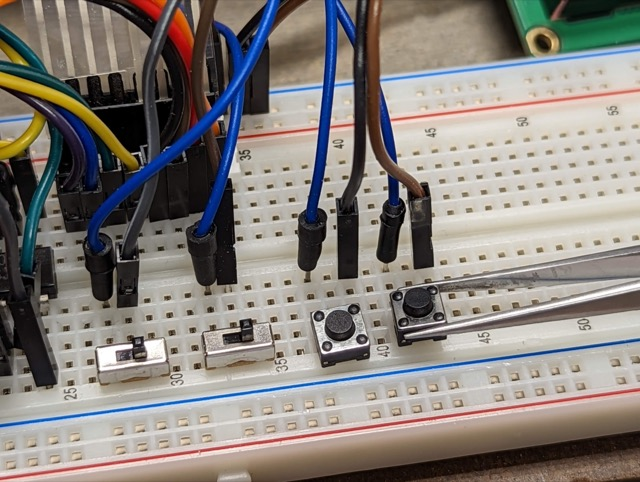
\includegraphics[height=4cm]{reconfiguration_images/remove_button}
        \label{fig:removeButton}
    }
    \hfil
    \subfloat[Inserting the piezodisc.]{
        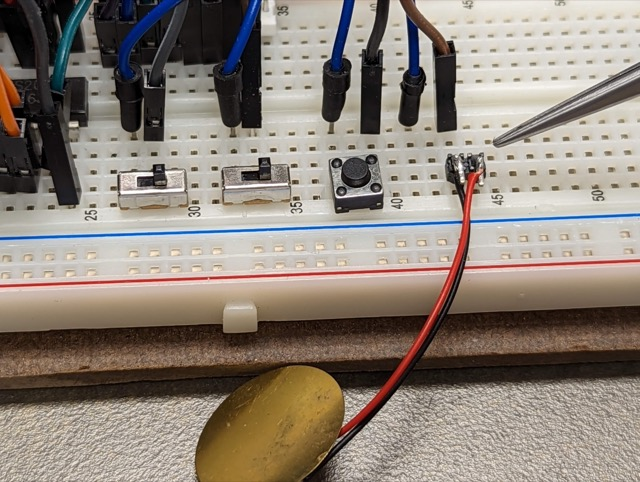
\includegraphics[height=4cm]{reconfiguration_images/insert_piezo}
        \label{fig:insertPiezo}
    }
    \hfil
    \subfloat[Adjusting the wiring for the piezodisc.]{
        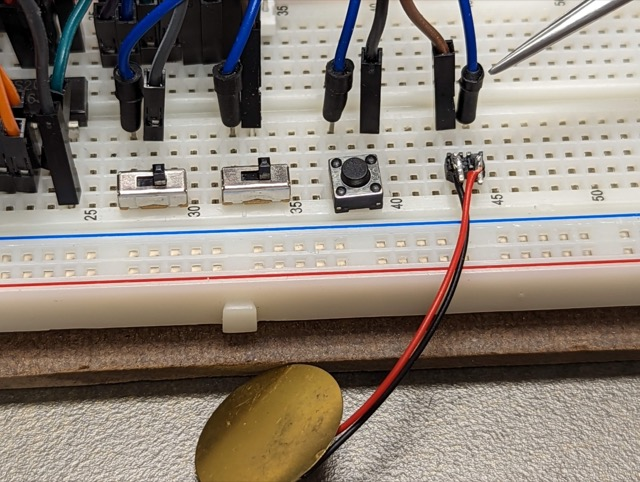
\includegraphics[height=4cm]{reconfiguration_images/adjust_piezo_wire}
        \label{fig:adjustPiezoWire}
    }
    \caption{Connecting the Piezoelectric Disc.
        The tweezers in these photos are to point out the changes and are not needed for \textit{these} modifications.}
\end{figure}

The piezodisc is now connected to the \developmentboard's pin D9, which is the pin that the right pushbutton used to be connected to.
The starter code will re-configure this pin to be an output pin.

\subsection{Connecting the ultrasonic echo sensor}

\begin{figure}
    \centering
    \subfloat[Locating the wires to remove.]{
        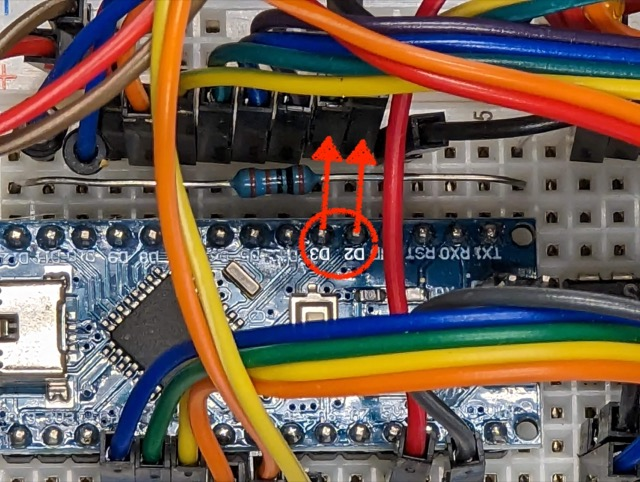
\includegraphics[height=4cm]{reconfiguration_images/pins_D2_D3}
        \label{fig:locateD2D3}
    }
    \\
    \subfloat[Removing the wire from contact point j10.]{
        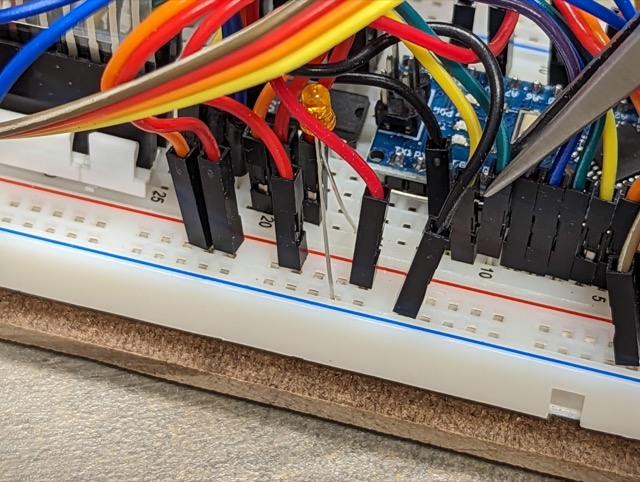
\includegraphics[height=4cm]{reconfiguration_images/remove_D3}
        \label{fig:removeD3}
    }
    \hfil
    \subfloat[Removing the wire from contact point j11.]{
        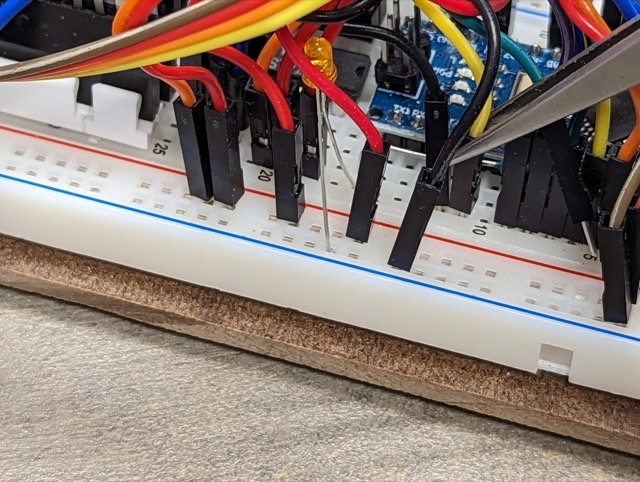
\includegraphics[height=4cm]{reconfiguration_images/remove_D2}
        \label{fig:removeD2}
    }
    \hfil
    \subfloat[An option is to leave the two wires hanging loosely.]{
        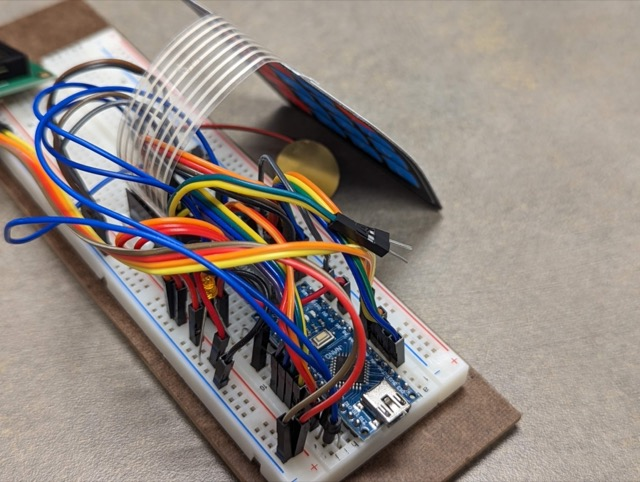
\includegraphics[height=4cm]{reconfiguration_images/NAND_wires_floating}
        \label{fig:nandFloat}
    }
    \hfil
    \subfloat[An option is to remove the wires completely from the breadboard.]{
        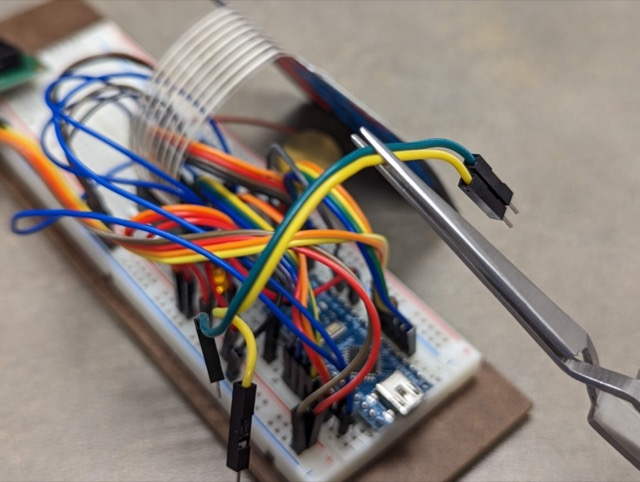
\includegraphics[height=4cm]{reconfiguration_images/NAND_wires_removed}
        \label{fig:nandRemoved}
    }
    \caption{Disconnecting the 74LS20 from the \developmentboard.}
\end{figure}

The \developmentboard's pins D2 \& D3 are currently used for the NAND values of the pushbuttons and of the keypad columns.
In the group project, we will use those pins for the ultrasonic echo sensor.

\subsubsection{Disconnecting the NAND} \label{subsubsec:disconnectNAND}

\textbf{\textit{Make sure that both you and your partner agree with which wires to pull before you do so!}}
If your partner is not available, then find someone to agree that you are about to pull the correct wires.

If you do not have the finger dexterity to remove the wires in the following steps with your fingertips, then the TAs will have a pair of needle-nose pliers during lab time that you can use.

\begin{description}
    \checkoffitem{Locate the wires that are connected to the \developmentboard's pins D2 \& D3 (Figure~\ref{fig:locateD2D3}).
        These are the wires in the breadboard's contact points j10 \& j11.}
    \checkoffitem{Gently remove the wire in the breadboard's contact point j10 (Figure~\ref{fig:removeD3}).}
    \checkoffitem{Gently remove the wire in the breadboard's contact point j11 (Figure~\ref{fig:removeD2}).}
    \checkoffitem{You may leave those two wires hanging loosely among the rat's nest of jumper wires, provided that they are positioned so they do not contact other components (Figure~\ref{fig:nandFloat}).
        Alternatively, you may \textit{very} gently tug at those two wires to completely remove them from the breadboard (Figure~\ref{fig:nandRemoved}).
        If you completely remove the wires, you can re-use them in Section~\ref{subsubsec:connectingSensor} to connect the ultrasonic echo sensor to the power and ground rails.}
\end{description}

\begin{figure}
    \centering
    \subfloat[Inserting a wire into contact point j11.]{
        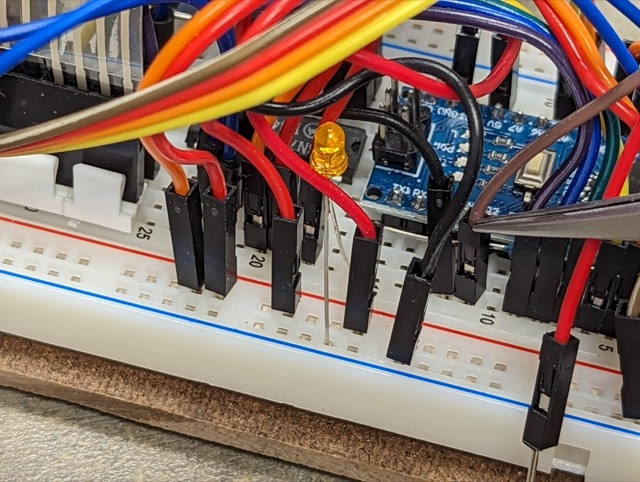
\includegraphics[height=4cm]{reconfiguration_images/insert_D2}
        \label{fig:insertD2}
    }
    \hfil
    \subfloat[Inserting a wire into contact point j10.]{
        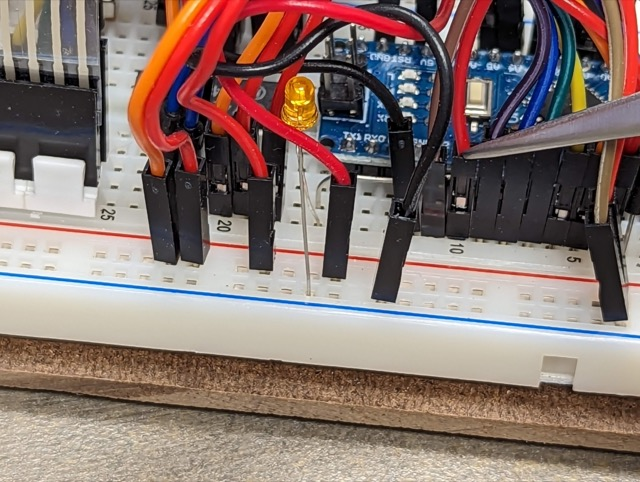
\includegraphics[height=4cm]{reconfiguration_images/insert_D3}
        \label{fig:insertD3}
    }
    \hfil
    \subfloat[The two 20cm wires, ready to be used.]{
        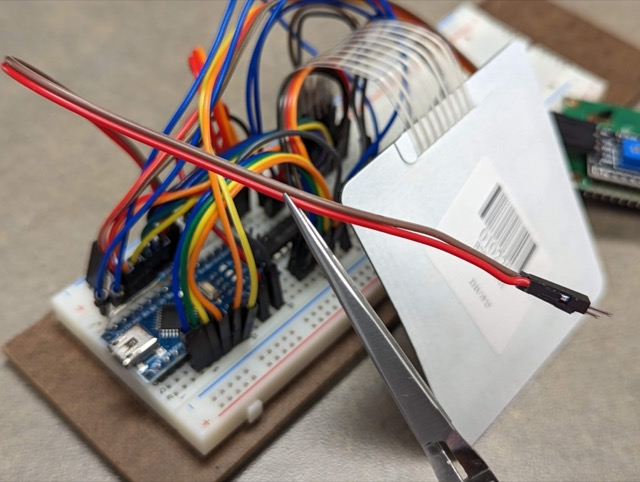
\includegraphics[height=4cm]{reconfiguration_images/20cm_D2_D3}
%        \label{fig:20cmD2D3}
    }
    \caption{Connecting the 20cm wires to the \developmentboard.}
\end{figure}

\subsubsection{Connecting the ultrasonic echo sensor} \label{subsubsec:connectingSensor}

You will first replace the NAND wires with 20cm male-to-male wires.

\begin{description}
    \checkoffitem{Insert a 20cm wire into contact point j11 (Figure~\ref{fig:insertD2}).
        Make a note of the wire's color for future reference.
        This is your \textbf{D2 wire}.}
    \checkoffitem{Insert a 20cm wire into contact point j10 (Figure~\ref{fig:insertD3}).
        Make a note of the wire's color for future reference.
        This is your \textbf{D3 wire}.}
\end{description}

Take a look at the ultrasonic echo sensor (Figure~\ref{fig:ultrasonic}).
Notice that it has four pins, labeled \texttt{Gnd}, \texttt{Echo}, \texttt{Trig}, and \texttt{Vcc}.

\begin{figure}
    \centering
    \subfloat[The back side of the ultrasonic sensor.]{
        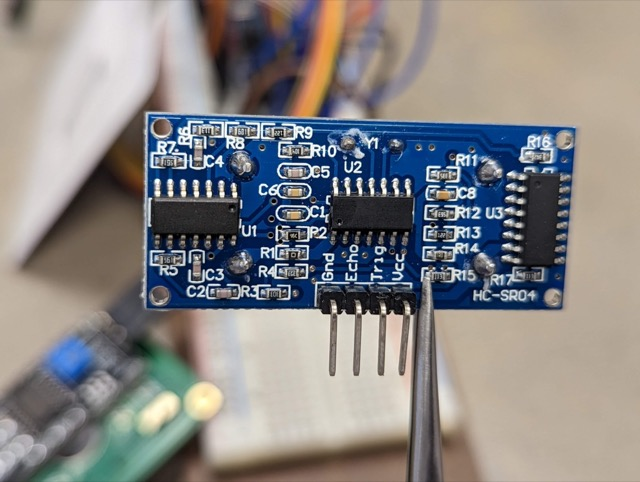
\includegraphics[height=4cm]{reconfiguration_images/ultrasonic_rear}
%        \label{fig:ultrasonicRear}
    }
    \hfil
    \subfloat[The front side of the ultrasonic sensor.]{
        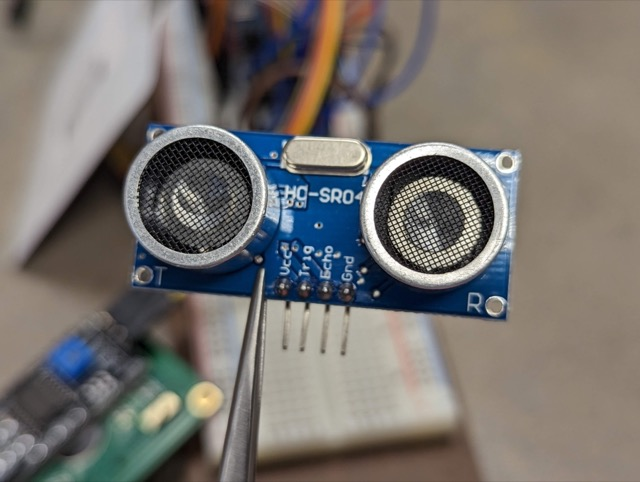
\includegraphics[height=4cm]{reconfiguration_images/ultrasonic_front}
%        \label{fig:ultrasonicFront}
    }
    \caption{The ultrasonic echo sensor. \label{fig:ultrasonic}}
\end{figure}

\begin{description}
    \checkoffitem{Insert the ultrasonic echo sensor in the breadboard's contact points d55--d58 (Figure~\ref{fig:ultrasonicInserted} shows the sensor in contact points e55--e58; however, testing shows slightly better results if the sensor's circuit board isn't allowed to dip into the breadboard's central channel).
        The \texttt{Gnd} pin should be in contact point d55, and the \texttt{Vcc} pin should be in contact point d58.
        The ultrasonic transducers should point toward the upper power/ground rails.}
    \checkoffitem{Insert the D2 wire into the breadboard's contact point b57, and the D3 wire into the breadboard's contact point b56 (Figure~\ref{fig:ultrasonicD2D3}).}
    \checkoffitem{Insert one end of a male-to-male wire in contact point b55 and the other end in the upper \ground.
        Insert one end of another male-to-male wire in contact point b58 and the other end in the upper \power.
        See Figures~\ref{fig:ultrasonicPwrGnd}--\ref{fig:pwrGnd}.
        If you fully-removed the wires between the 74LS20 and the \developmentboard\ in Section~\ref{subsubsec:disconnectNAND} then you can use those wires for this step (as we did in the photographs);
        otherwise, you will to use spare wires from your hardware kit.
        For best performance, position these wires so that they are not directly in front of the ultrasonic transducers.}
\end{description}

\begin{figure}
    \centering
    \subfloat[The back side of the ultrasonic sensor.]{
        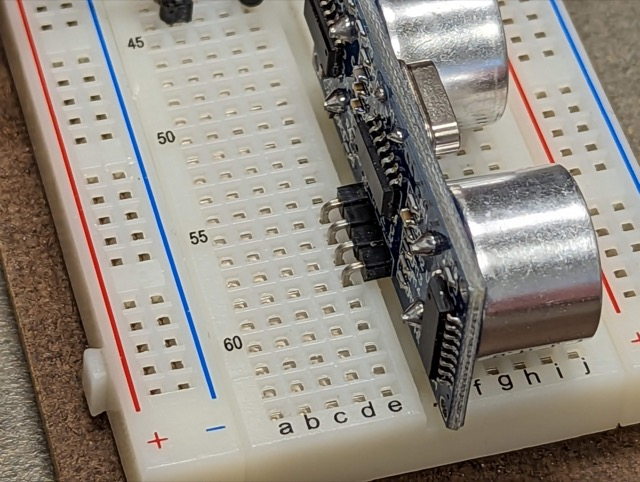
\includegraphics[height=4cm]{reconfiguration_images/ultrasonic_inserted}
        \label{fig:ultrasonicInserted}
    }
    \hfil
    \subfloat[The front side of the ultrasonic sensor.]{
        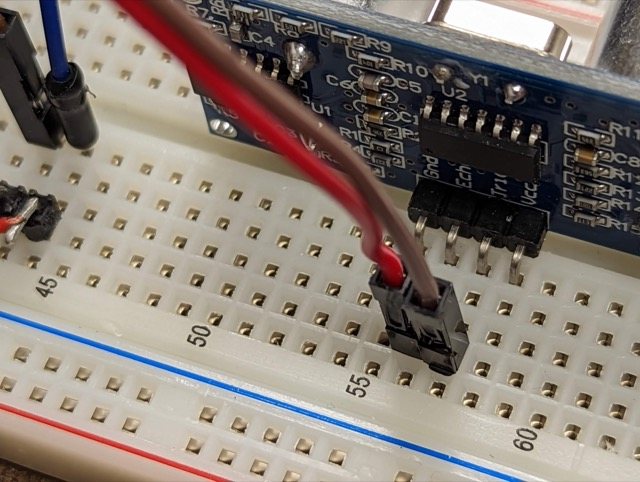
\includegraphics[height=4cm]{reconfiguration_images/ultrasonic_D2_D3}
        \label{fig:ultrasonicD2D3}
    }
    \hfil
    \subfloat[Inserting one end of the power and ground wires.]{
        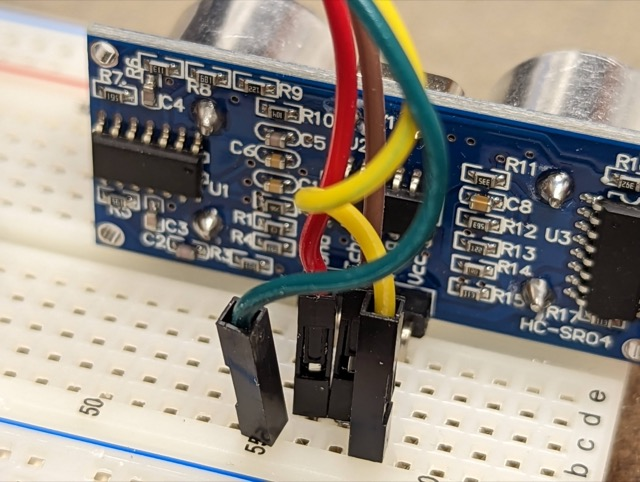
\includegraphics[height=4cm]{reconfiguration_images/ultrasonic_pwr_gnd}
        \label{fig:ultrasonicPwrGnd}
    }
    \hfil
    \subfloat[Inserting the other end of the power and ground wires in the power and ground rails.]{
        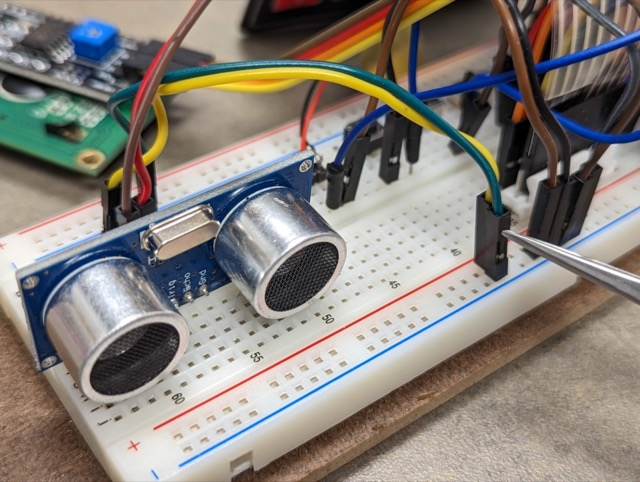
\includegraphics[height=4cm]{reconfiguration_images/pwr_gnd}
        \label{fig:pwrGnd}
    }
    \caption{Connecting the ultrasonic echo sensor.}
\end{figure}

The ultrasonic echo sensor is now connected to the \developmentboard's pins D2 \& D3.
The starter code will re-configure D2 to be an output pin.

\begin{figure}
    \centering
    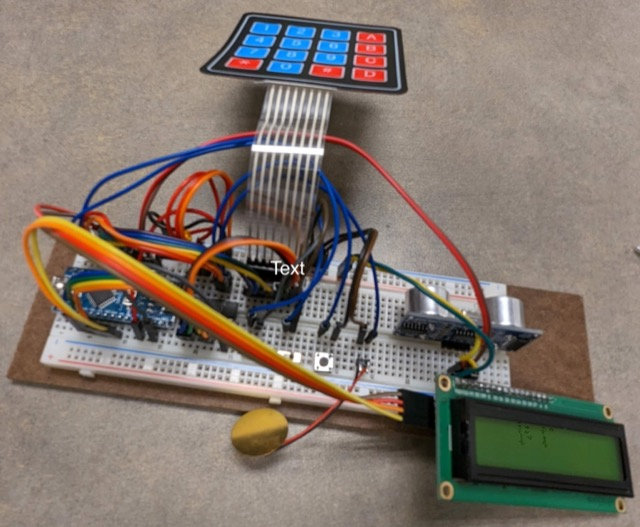
\includegraphics[width=10cm]{reconfiguration_images/complete}
    \caption{The Cow Pi circuit with modfications complete.}
\end{figure}

\vspace{1cm}

Your Cow Pi circuit is now ready for you to design and code the software for a range finder and alarm.


    \section{System Specification} \label{sec:spec}                     %! suppress = LabelConvention
\begin{enumerate}
    \item Definitions
        \begin{description}
            \item[Threshold Range] The distance at which a detected object will cause the system to produce an audible alarm
            \item[Strobe] An illumination of an LED for 50ms
            \item[Chirp] A 5kHz tone lasting 50ms
        \end{description}
    \item \label{spec:modes} The slide-switches shall control the mode of operation.
        \begin{enumerate}
            \item Both switches in the \textit{left position}: Normal Operation
            \item The \textbf{left switch} in the \textit{right position} and the \textbf{right switch} in the \textit{left position}: Single-Pulse Operation
            \item Both switches in the \textit{right position}: Threshold Adjustment
            \item The \textbf{left switch} in the \textit{left position} and the \textbf{right switch} in the \textit{right position}: Continuous Tone
        \end{enumerate}
    \item \label{spec:continuousTone} When the range finder and alarm system is in \textbf{Continuous Tone} mode:
        \begin{enumerate}
            \item The system shall not detect the range of nearby objects: it shall neither emit nor detect ultrasound
            \item The system shall not illuminate an LED
            \item The system shall produce a continuous 5kHz audible tone
        \end{enumerate}
    \item \label{spec:thresholdAdjustment} When the range finder and alarm system is in \textbf{Threshold Adjustment} mode:
        \begin{enumerate}
            \item The system shall not detect the range of nearby objects: it shall neither emit nor detect ultrasound
            \item The system shall not produce an audible tone
            \item The system shall not illuminate an LED
            \item The system shall prompt the user on the \textbf{display module} to enter the threshold range, in centimeters
                \begin{itemize}
                    \item You may assume that the user understands what the system does: the prompt must be \textit{meaningful}, but it may be \textit{succinct}
                \end{itemize}
            \item The user shall be able to enter the threshold range, in centimeters, using the numeric keypad
                \begin{enumerate}
                    \item The user will enter the range in decimal
                    \item The system shall echo the user's input, digit-by-digit, on the \textbf{display module} as they type their input
                    \item The user will indicate that they have finished entering their input by pressing the `\#' key
                \end{enumerate}
            \item After the user has completed their input, then any value less than 50cm or greater than 400cm shall be rejected as an invalid threshold;
                the system shall display a helpful error message on the \textbf{display module} and re-prompt the user to enter the threshold range
            \item After the user has completed their input, and if the input is valid, then the system shall display ``Threshold (value)cm'' on the \textbf{display module}, where ``(value)'' shall be the numeric threshold range in centimeters;
                this shall be displayed until the user takes the system out of the Threshold Adjustment mode
        \end{enumerate}
    \item \label{spec:singlePulseOperation} When the range finder and alarm system is in \textbf{Single-Pulse Operation} mode: \\
        {\footnotesize Note: the references here to ``the pushbutton'' refer to the Cow Pi's original \textbf{left pushbutton}}
        \begin{enumerate}
            \item The system shall neither emit nor receive ultrasound, shall not produce an audible tone, and shall not illuminate an LED, \textit{until} the pushbutton has been pressed
            \item Whenever the user presses the \textbf{pushbutton}, the system shall emit one ultrasonic pulse
            \item If the system does not receive that pulse's echo, the system shall resume waiting for the user to press the pushbutton
            \item \label{spec:singlePulseResponse} If the system does receive that pulse's echo:
                \begin{enumerate}
                    \item The system shall strobe both LEDs once
                    \item If the object's distance is less than the threshold range then the system shall emit one chirp
                    \item The system shall then resume waiting for the user to press the pushbutton
                \end{enumerate}
        \end{enumerate}
    \item \label{spec:normalOperation} When the range finder and alarm system is in \textbf{Normal Operation} mode, the system shall repeatedly:
        \begin{enumerate}
            \item \label{spec:emitUltrasound} Emit an ultrasonic pulse and take no further action until either the system receives an echo or the system can establish that it will not receive an echo
            \item If the system can establish that it will not receive an echo:
                \begin{enumerate}
                    \item The system shall stop strobing the LEDs and chirping if it previously was doing so
                    \item The system shall repeat the action in Requirement~\ref{spec:emitUltrasound}
                        {\footnotesize
                        \begin{itemize}
                             \item Repeating the action may be postponed until after necessary quiescent periods
                        \end{itemize}}
                \end{enumerate}
            \item If the system receives an echo:
                \begin{enumerate}
                    \item The system shall compute and display the object's distance, in centimeters
                    \item The system shall compute and display the object's rate of approach, in centimeters per second
                    \item The system shall strobe both LEDs at the rate described by Table~\ref{tab:alarmPeriods}
                    \item If the object's distance is less than the threshold range, the system shall emit chirps at the rate described by Table~\ref{tab:alarmPeriods}
                    \item After the system has completed the speed and distance calculations, it shall repeat the action in Requirement~\ref{spec:emitUltrasound}
                        {\footnotesize
                        \begin{itemize}
                            \item Repeating the action may be postponed until after necessary quiescent periods
                        \end{itemize}}
                \end{enumerate}
        \end{enumerate}
    \item All mechanical inputs shall be properly debounced
    \item The system shall always be responsive to user input
        \begin{itemize}
            \item The user will never press two keys on the numeric keypad at the same time
            \item The system may ignore changes to the slide-switches while the user enters a new threshold range
            \item The system may block while displaying an error message
            \item But for those exceptions, there shall be no noticeable lag when responding to an input
        \end{itemize}
\end{enumerate}

\begin{table}
    \centering
    \begin{tabular}{||c|c|c|c||} \hline\hline
        \multirow{2}{*}{distance}   & LEDs on /         & LED off /         & total     \\
                                    & Piezo sounding    & Piezo silent      & period    \\ \hline\hline
        $distance \geq 250cm$          & $50ms$            & $2450ms$          & $2500ms$  \\ \hline
        $200cm \leq distance < 250cm$  & $50ms$            & $1950ms$          & $2000ms$  \\ \hline
        $150cm \leq distance < 200cm$  & $50ms$            & $1450ms$          & $1500ms$  \\ \hline
        $100cm \leq distance < 150cm$  & $50ms$            & $ 950ms$          & $1000ms$  \\ \hline
        $ 50cm \leq distance < 100cm$  & $50ms$            & $ 700ms$          & $ 750ms$  \\ \hline
        $ 25cm \leq distance <  50cm$  & $50ms$            & $ 450ms$          & $ 500ms$  \\ \hline
        $ 10cm \leq distance <  25cm$  & $50ms$            & $ 200ms$          & $ 250ms$  \\ \hline
        $distance < 10cm$           & $50ms$            & $  75ms$          & $ 125ms$  \\ \hline\hline
    \end{tabular}
    \caption{Strobe and Chirp periods for various distances to an object}\label{tab:alarmPeriods}
\end{table}

    \section{Initial Software Changes} \label{sec:initialSoftware}      \subsection{Examining the Starter Code}

\paragraph{user\_controls.c}
The \function{initialize_controls()} function is where you'll place any alarm-related code that needs to be run once when the program starts.
The \function{manage_controls()} function is where you'll place any alarm-related code that needs to run with every iteration of the program's main loop.
You may, of course, add helper functions.

\paragraph{shared\_variables.h}
This is the only header file you will turn in, so if you need to share any \lstinline{enum}s, \lstinline{struct}s, or variables between \textit{.c} files, place them in here and not in the other header files, so that we can compile your code.
When you need to share a variable between \textit{.c} files, declare it in exactly one \textit{.c} file (preferably the one that the variable best coheres to) without the \lstinline{extern} keyword,
and then externalize it by declaring it again with the \lstinline{extern} keyword in \textit{shared\_variables.h}.
This approach will create just one global symbol for the variable in the program while making it ``visible'' to the code in the other \textit{.c} files.

\subsection{A Quick Note about Creating State Machines}

A not-uncommon pattern in embedded systems is to design the system as a state machine, or as multiple state machines.
The states are represented as the value of an enumerated type.
A couple of key advantages of writing the system as a state machine or as a collection of state machines is that it's easy to change the state based on inputs,
and it's easy for the parts of the system that take action to do so based on what state the state machine is in.

\subsection{Read the Switches}

\begin{figure}[h]
    \centering
    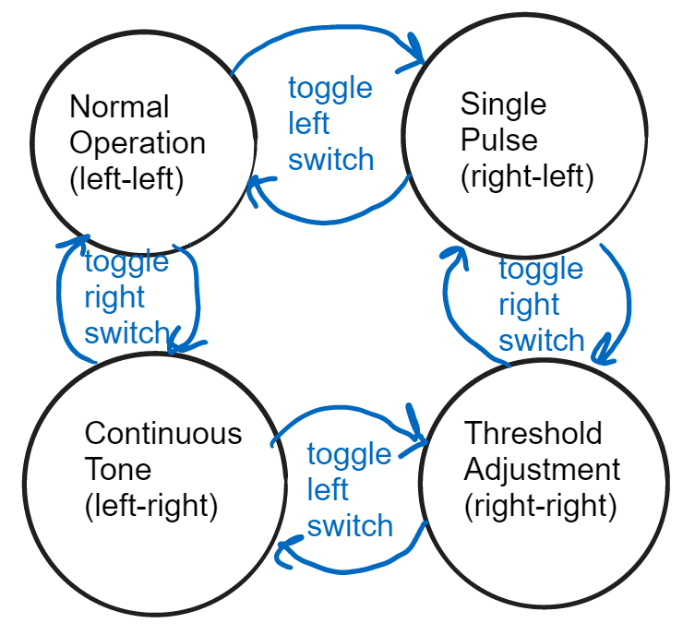
\includegraphics[width=3in]{modeStateMachine}
    \caption{\label{fig:modeStateMachine} State machine describing the rangefinder's modes of operation.}
\end{figure}

Create a way to track which mode the system is in (Requirement~\ref{spec:modes}).
Be sure to declare it not only in \textit{user\_controls.c} (without the \lstinline{extern} modifier) but also in \textit{shared\_variables.h} (with the \lstinline{extern} modifier).
Add code to \function{manage_controls()} to poll the positions of the slide-switches and set the system's mode accordingly.

\subsection{Read the Pushbutton} \label{subsec:readPushbutton}

As noted in Requirement~\ref{spec:singlePulseOperation}, if the system is in Single-Pulse Operation mode and the user presses the left pushbutton, they want to emit exactly one ultrasound pulse to get the distance to an object.
\begin{figure}[h]
    \centering
    \includegraphics[width=10cm]{internet_images/one_ping_only}
    \caption{Verify our range to target. One ping only. \\ \tiny Image by Paramount Pictures Corporation \label{fig:onePingOnly}}
\end{figure}

Create a variable to indicate that the user has requested a ping.
Be sure to declare it not only in \textit{user\_controls.c} (without the \lstinline{extern} modifier) but also in \textit{shared\_variables.h} (with the \lstinline{extern} modifier).
Add code to \function{initialize_controls()} to set this variable initially to \lstinline{false}.
Add code to \function{manage_controls()} to set this variable to \lstinline{true} when and only when the use presses the button while in Single-Pulse Operation mode.
The variable should be set to \lstinline{true} only \textit{once} per press.
(Do \textit{not} set it to \lstinline{true} just because the user is still holding the button down.)

Do not worry about setting this variable to \lstinline{false} yet;
that will come later.

\vspace{1cm}

You can now continue to work through the remainder of the lab with your partner, perhaps pair programming,
or you can decide to have one partner work on Section~\ref{sec:distance} and the other work on Section~\ref{sec:sound}.
Regardless, you will need to work together on Section~\ref{sec:integration}, as this is when you will integrate the work from Sections~\ref{sec:distance}--\ref{sec:sound}.


%    \section{Measuring Distance and Speed} \label{sec:distanceAndSpeed} \input{distance_speed}

    \section{Measuring Distance} \label{sec:distance}                   You will use the ultrasonic echo sensor to determine the distance to an object.

\subsection{Theory of Operation}

The ultrasonic echo sensor has a simple interface.
If your program places a logic-high signal on the \lstinline{TRIGGER} pin for 10\textmu s and then drop it to logic-low, then the device will emit a short burst of ultrasound.
The device will then raise the \lstinline{ECHO} pin's logic level to high.
If there is a nearby object, the ultrasound will reflect off of it, and the sensor will detect the echo.
After detecting the echo, the device will drop the \lstinline{ECHO} pin's logic level to low.
If no echo is received, then the device will eventually time-out and drop the \lstinline{ECHO} pin's logic level to low.
After affording the device a quiescent period, the cycle can be repeated.

%Various datasheets\footnote{
%    \url{https://cdn.sparkfun.com/datasheets/Sensors/Proximity/HCSR04.pdf}}$^,$\footnote{\url{https://web.eece.maine.edu/~zhu/book/lab/HC-SR04\%20User\%20Manual.pdf}}$^,$\footnote{\url{https://www.handsontec.com/dataspecs/HC-SR04-Ultrasonic.pdf}
%}\ differ slightly in a few particulars.
%Some describe the time-out period as 36ms, others 38ms.
%Some describe the quiescent period as at least 10ms after the \texttt{Echo} pin's logic drops low; others recommend at least 60ms after the \texttt{Echo} pin's logic goes high.
%The datasheets generally agree that under typical conditions, the device will be able to detect an echo from a $0.5\mathrm{m}^2$ target within 4~meters of the sensor.
%One datasheet suggests that under some conditions, this distance may be as great as 5~meters.\footnote{
%    During testing of the sample solution, sometimes objects 250cm away couldn't always be reliably detected; at other times I was able to detect objects up to 320cm away.
%}

If your program measures the time between the \lstinline{ECHO} pin's logic going high and subsequently going low, then it knows how long the ultrasound travelled to the object and back again.
The classical relationship $distance = speed \times time$ requires that we know how fast the ultrasound travels.

The speed of sound depends on the medium it travels through and the temperature of that medium.
We will assume the medium is air.
\begin{description}
    \item[Old Hardware] If you are using the old hardware, you may assume that the air temperature is 70\degree~Fahrenheit (21.1\degree~Celsius). %21\degree~Celsius (69.8\degree~Fahrenheit).
        The speed of sound for 70\degree\ air is $348.8\frac{m}{s}$.\footnote{
            \url{https://www.weather.gov/epz/wxcalc_speedofsound}
        }
%        The speed of sound for 21\degree\ air is $343.72\frac{m}{s}$.\footnote{
%            \url{https://www.weather.gov/epz/wxcalc_speedofsound}
%        }
    \item[New Hardware] If you are using the new hardware, you will treat the speed of sound as a function air temperature.
        Assuming the temperature $T$ is measured in \degree C, the speed of sound in air is\footnote{
        \url{https://www.weather.gov/media/epz/wxcalc/speedOfSound.pdf}
        }
        \[
%            643.855 \times \sqrt{1 + \frac{T}{273.15}} \times 0.5144444
            331.228 \times \sqrt{1 + \frac{T}{273.15}} \frac{m}{s}
        \]
\end{description}

Thus, by knowing the round-trip travel time, we can determine the distance that the ultrasonic pulse travelled.
The distance to the object it echoed off of will be half of the round-trip distance.

\subsection{The Wrong Calculation}

The internet is littered with example code for measuring distance that instructs you to divide the ultrasonic pulse's round-trip travel time by 58 to obtain the distance in centimeters.
Few of these explain the origin of that particular calculation; however, if you look carefully, you can find one that does.\footnote{
    \url{https://docs.arduino.cc/built-in-examples/sensors/Ping/}
}
Like approximating gravitational acceleration as $10\frac{m}{s^2}$, the calculation of ``divide microseconds by 58'' is simple enough for someone to easily use and provides an adequate approximation.
Like approximating gravitational acceleration as $10\frac{m}{s^2}$, the calculation of ``divide microseconds by 58'' provides you with the wrong answer if ``approximately correct'' is insufficient.

The errors stem from three sources:
\begin{enumerate}
    \item The formulation states that the speed of sound is $340\frac{m}{s}$, but this is the case only when the air temperature is 14.66\degree~Celsius (58.4\degree~Fahrenheit).
        While there are situations in which that \textit{will} be the air temperature, students using the new hardware will measure the temperature, and students using the old hardware will assume the temperature is the thermostat set-point for Avery Hall.
    \item Even if the temperature were 14.66\degree~Celsius, the formulation approximates the speed of sound as $\frac{1}{29}\frac{\mu s}{cm}$, but $\left(340\frac{m}{s}\right)^{-1} = \frac{1}{29.41}\frac{\mu s}{cm}$.
        This rounding error adds up quickly.
    \item On the ATmega328P microcontroller (which most of the examples are targeting), the timer typically used to measure time is only accurate to within 4\textmu s.
        Even if $\frac{1}{29}\frac{\mu s}{cm}$ were the correct expression, this will produce an error of about 1mm.
        If we were using floating point arithmetic, this could be dismissed as a rounding error, but we are using integer arithmetic.
        Because integer division truncates the fractional portion of the quotient, there will be times in which ``round-towards-zero'' produces an error of a full centimeter relative to the answer that a more-careful computation would have produced.
\end{enumerate}


\subsection{The Correct Calculation}

\subsubsection{Practical Considerations}

\paragraph{Arithmetic}

As neither of our microcontrollers have a floating point unit (FPU), we want to avoid floating point calculations, which are computationally expensive when performed entirely in software.
Further, the ATmega328P cannot perform division in hardware, and so we want to avoid integer division unless the divisor is a power of two when using the old hardware.
The RP2040 has an integer divider that requires 8 processor clock cycles to perform division, so we might allow integer division with the new hardware -- but we have an equation that will not require the integer divider.

\paragraph{Time}

After we configure a timer to manage the sensor, we will be able to use its counter to determine the round-trip travel time.
On the old hardware, the ``tick'' will be a half-microsecond.
On the new hardware, the ``tick'' will be one microsecond.

\subsubsection{The Equations}\label{subsubsec:equations}

These equations can be used to accurately compute the distance to an object.
That is, the computed distance is half of the ultrasonic pulse's round-trip distance.
The derivation of these equations can be found in Appendix~\ref{sec:distanceFormulation}.

\paragraph{Old Hardware}

\[
    distance = time_{\mathrm{half}\mu s} \times \frac{18,025 cm}{\mathrm{half}\mu s} \div 2^{21}
\]

Even though $distance$ will be less than 500~cm, you will need at least 31 bits to represent the intermediate products when performing the arithmetic.

\paragraph{New Hardware}

\[
    distance = time_{\mu s} \times \left( 256,108,888 - 121,907 \times ADC\_register\_value \right) \frac{cm}{\mu s} \div 2^{33}
\]

Even though $distance$ will be less than 500~cm, you will need at least 44 bits to represent the intermediate products when performing the arithmetic.

\textcolor{red}{Obtaining the $ADC\_register\_value$ will be treated as extra credit.
If you do not wish to pursue that extra credit, then you may hard-code $ADC\_register\_value$ as 889, which is the value corresponding to 21.05\degree C (69.9\degree F).}

%There is also a practical consideration with respect to the sensor itself.
%Sound isn't particularly directional.
%The horns surrounding the ultrasonic transducers help to limit the ``beam width,'' but only to a degree.
%Pointing the sensor straight down an otherwise empty hallway, you will probably still detect a reflection from the walls to either side.\footnote{
%    If you're feeling nerdy, you could use right-angle trigonometry to determine the ``beam width'' --
%    point the sensor straight at a wall to determine how far away from it you are (the ``opposite''), then point the sensor parallel to the wall and take a reading (the hypoteneuse).
%    Divide the ``opposite'' by the hypoteneuse and take the arcsin -- the resulting value is the angle from straigth-ahead to how far to the right/left the sensor will detect a reflection.
%}



\subsection{Examining the Starter Code}

The \function{initialize_sensor()} function is where you'll place any alarm-related code that needs to be run once when the program starts.
The \function{manage_sensor()} function is where you'll place any alarm-related code that needs to run with every iteration of the program's main loop.
You will, of course, add code outside these functions too: an interrupt service routine for a timer, an interrupt handler for the distance sensor, and possibly helper functions.

\subsection{Single-Pulse Operation} \label{subsec:distanceSinglePulseOperation}

\begin{description}
    \checkoffitem{Create a variables to:
        \begin{itemize}
            \item indicate whether an object has been detected
            \item indicate the object's distance (if the object is detected)
            \item indicate the object's rate of approach (this will only be useful in Normal Operation mode)
        \end{itemize}
        Be sure to declare them not only in \textit{sensor.c} (without the \lstinline{extern} modifier) but also in \textit{shared\_variables.h} (with the \lstinline{extern} modifier).
    }
    \checkoffitem{In \function{initialize_sensor()}, initialize the object detection variable to indicate that an object has not been detected.}
\end{description}

A fully-correct implementation of Single-Pulse Operation mode has the alarm chirp if an object is detected closer than the threshold range (Requirement~\ref{spec:singlePulseOperation}).
For now, your focus will be on determining the distance to an object.

\begin{description}
    \checkoffitem{In \textit{sensor.c}, create a temporarily-empty interrupt handler that will be used to respond to the sensor timer's interrupts.
        Don't forget to pre-declare this functions above \function{initialize_sensor()}.}
    \checkoffitem{In \function{initialize_sensor()}, register that function as an ISR for a timer interrupt that has a period of 32,768\textmu s}
        \begin{itemize}
            \item On the old hardware, use TIMER1.
            \item On the old hardware, this should configure TIMER1 to have a ``tick'' of $\frac{1}{2}\mu s$ (which we will refer to as $1\mathrm{half}\mu s$).
                On the new hardware, the timer's ``tick'' will be $1\mu s$
        \end{itemize}
\end{description}

%Using the ``Timers'' section of the Cow Pi datasheet,\footnote{
%    \url{https://cow-pi.readthedocs.io/en/latest/microcontroller.html\#timers}
%}
%place code in \function{initialize_sensor()} to configure Timer1 to produce an \textbf{overflow} interrupt every 32,768\textmu s, using the ``Normal'' mode.
%Place in \function{initialize_sensor()} code to enable that interrupt.

\begin{description}
    \checkoffitem{Create a state machine for the sensor that can be ``initial-start'', ``powering-up'', ``ready,'' ``active-listening,'' ``active-detected,'' and ``quiescent.''}
    \checkoffitem{Initialize that state machine to be ``initial-start''.}
\end{description}

\textit{If you are using the new hardware}, you will need to be able to read from an analog-digital converter (ADC).
\begin{description}
    \checkoffitem{Create a pointer to an \lstinline{adc_t} structure and point it to \lstinline{0x4004c000}.}
    \checkoffitem{In \function{initialize_sensor()}, configure the ADC using its \lstinline{control} register:}
        \begin{itemize}
            \item Set bit20 to \lstinline{1} indicating that we are interested in ADC channel 4.
            \item Set bits14..12 to \lstinline{4} indicating that channel 4 is the next channel to convert.
            \item Set bits1..0 to \lstinline{3} indicating that the temperature sensor should be powered, and that the ADC should be enabled.
        \end{itemize}
\end{description}


\begin{figure}[h]
    \centering
%    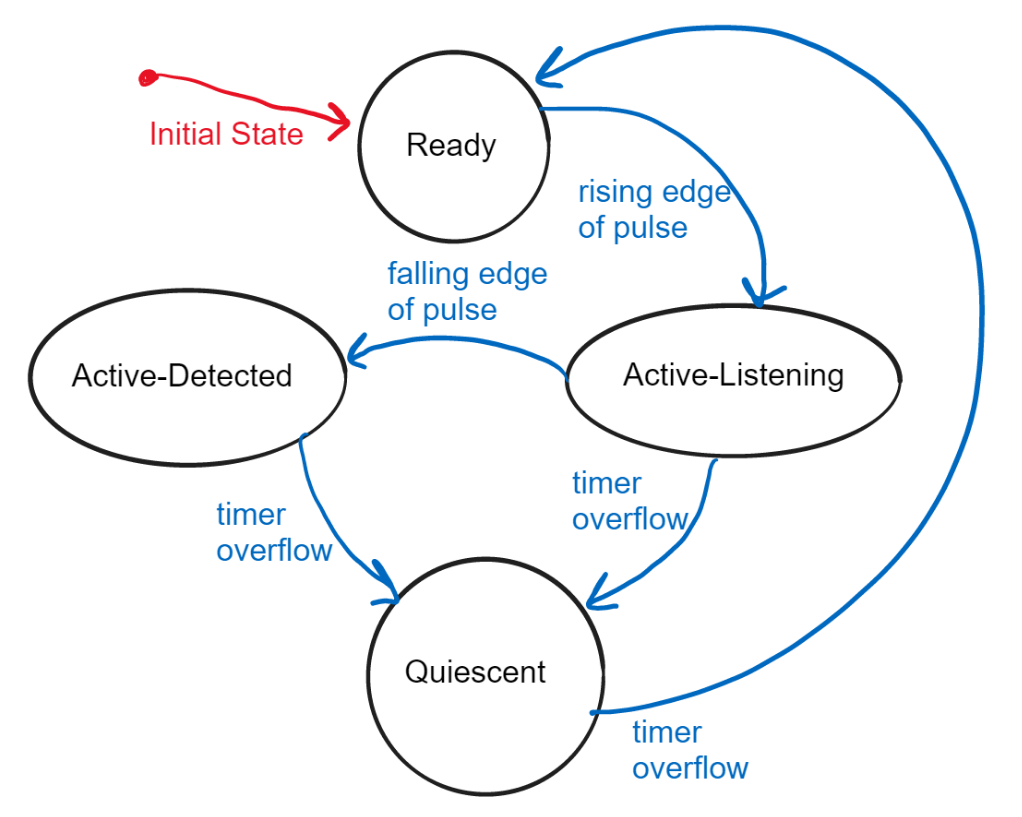
\includegraphics[width=3in]{sensorStateMachine}
    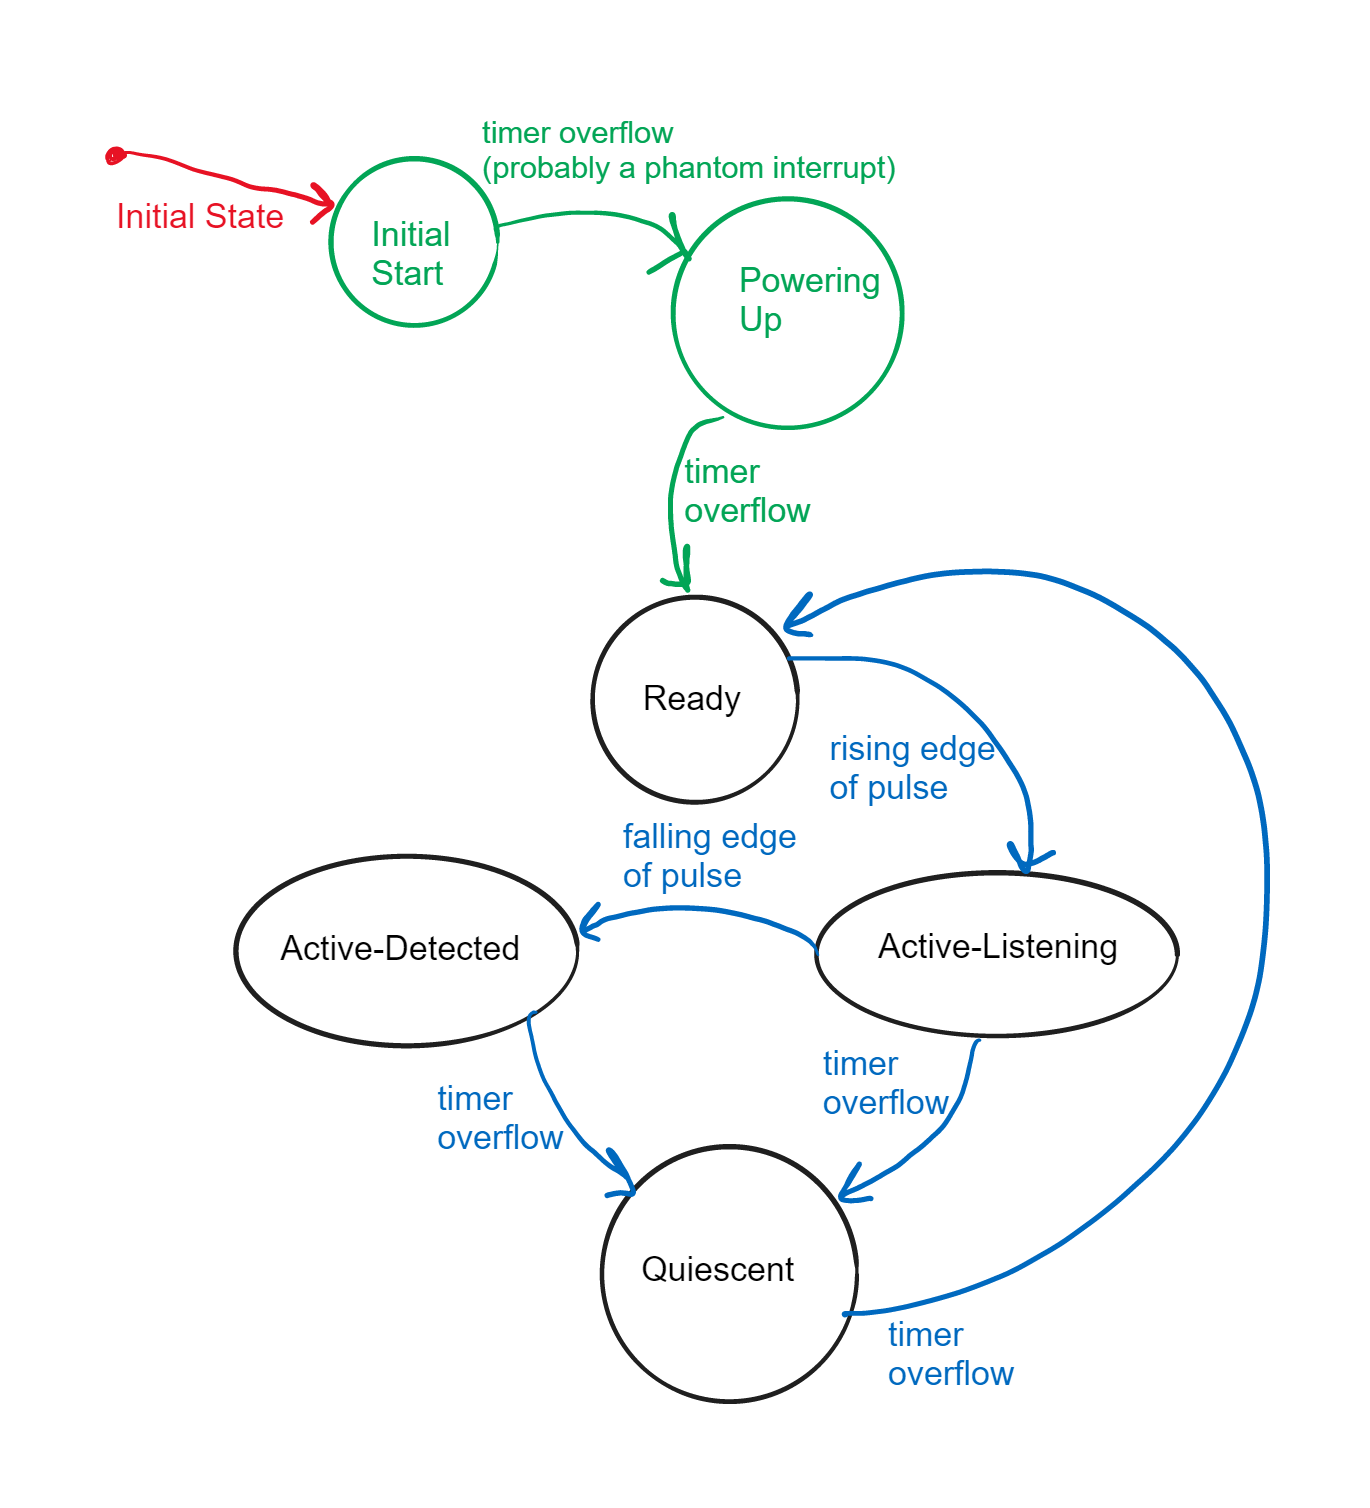
\includegraphics[width=4in]{noPhantomInterrupts}
    \caption{\label{fig:sensorStateMachine} State machine describing the control of the distance sensor.
%        See Appendix~\ref{sec:phantom} for an alternative state machine.
    }
\end{figure}

%Use the \function{ISR} macro to create an interrupt service routine in \textit{sensor.c} for that interrupt.
%Leave the ISR's body empty for now.

\begin{description}
    \checkoffitem{In \textit{sensor.c}, create a temporarily-empty interrupt handler that will be used to detect the rising and falling edge of the pulse. %one for actions to be taken when the sensor emits its ultrasound pulse, and one for actions to be taken when the sensor receives an echo.
        Don't forget to pre-declare this functions above \function{initialize_sensor()}.}
        \begin{itemize}
            \item \textcolor{red}{\textbf{Do \textit{NOT} use \function{manage_sensor()} as your interrupt handler!}}
        \end{itemize}
    \checkoffitem{Place in \function{initialize_sensor()} code to register the handler for a CHANGE on the \lstinline{ECHO} pin.}
\end{description}

\paragraph{Allow Time for the System to Initialize}

When the system starts up, the input pins and the timers may fire ``phantom'' interrupts.
We will handle this taking no action until the sensor timer has fired at least two interrupts.

In the timer interrupt handler:
\begin{description}
    \checkoffitem{If the sensor's state machine is in its ``initial-start'' state, place it in its ``powering-up'' state}
    \checkoffitem{If the sensor's state machine is in its ``powering-up'' state, place it in its ``ready'' state}
\end{description}

\paragraph{Initiate a Pulse}
Place code in \function{manage_sensor()} that, whenever a ping is requested (see Section~\ref{subsec:readPushbutton}), will:
\begin{description}
    \checkoffitem{First, set the \lstinline{TRIGGER} pin to logic-high}
    \checkoffitem{Then, set the variable indicating that a ping is requested to \lstinline{false}}
    \checkoffitem{Next, delay for 10\textmu s}
    \begin{description}
        \item[Old Hardware] \phantom{x} \\
        \begin{itemize}
            \item You will need a pointer to TIMER1
            \item Use the timer's counter to busy-wait for 20half\textmu s
        \end{itemize}
        \item[New Hardware] \phantom{x} \\
        \begin{itemize}
            \item You will need a pointer to the general-purpose timer
            \item Use the timer's counter to busy-wait for 10\textmu s
        \end{itemize}
    \end{description}
    \checkoffitem{Finally, set the \lstinline{TRIGGER} pin to logic-low}
\end{description}

Several microseconds later, the sensor will emit its ultrasound pulse and raise its \texttt{Echo} line to logic-high.

\paragraph{Handle the Start of a Pulse}
In the function that you registered to handle the pulse edges on the \lstinline{ECHO} pin, you want to keep track of whether the interrupt handler was triggered for a rising or falling edge.
While you \textit{could} do so by checking the logic level on the \lstinline{ECHO} pin, you can also assume that rising and falling edges alternate --
you will never have two rising edges in a row, and you will never have two falling edges in a row.

If the pin interrupt handler was triggered for a rising edge, you want to start the process of determining exactly how much time passes between emitting the pulse and receiving the echo.
\begin{description}
    \checkoffitem{First, reset the sensor timer's}
    \checkoffitem{Then, \textit{if you are using the new hardware}, copy the value of the timer's counter into a \lstinline{volatile} global variable}
        \begin{itemize}
            \item You will need a pointer to the general-purpose timer
            \item \textit{For the old hardware}, the timer's counter will be 0 after resetting the timer, so copying it is not necessary.
        \end{itemize}
    \checkoffitem{Finally, place the sensor state machine in its ``active-listening'' state}
\end{description}

Two things will happen in the next 38 (or fewer) milliseconds: the signal on the \lstinline{ECHO} pin will fall to logic-low, and the sensor timer will fire an interrupt.
Whichever happens first, the signal falling low or the timer interrupt, will tell us whether there's an object.

\paragraph{Handle the End of a Pulse}
If the signal on the \lstinline{ECHO} pin falls to logic-low first, then it's because there's an object that reflected the ultrasound pulse.

If the pin interrupt handler was triggered for a falling edge, and if the sensor is ``active-listening,'' then you want to capture the information needed to compute the distance.
\begin{description}
    \checkoffitem{First, copy the value of the timer's counter into a \lstinline{volatile} global variable}
        \begin{description}
            \item[Old Hardware] \phantom{x} \\
                \begin{itemize}
                    \item You will need a pointer to TIMER1
                    \item The value that you copy is the number of half-microseconds between the pulse emission and the echo's return
                \end{itemize}
            \item[New Hardware] \phantom{x} \\
                \begin{itemize}
                    \item You will need a pointer to the general-purpose timer
                    \item This value, minus the value you copied at the start of the pulse, is the number of microseconds between the pulse emission and the echo's return
                \end{itemize}
        \end{description}
    \checkoffitem{Then, place the sensor state machine in its ``active-detected'' state}
\end{description}

\paragraph{Handle Timer Interrupt}

If the sensor timer overflows before the signal on the \lstinline{ECHO} pin falls low, then there is not an object within detectable range.
The sensor will time-out after 36,000--38,000\textmu s, and the sensor timer will fire an interrupt after 32,768\textmu s.
Any object whose echo might have been detected after this must be beyond the sensor's detection range.

If the sensor is ``active-listening'' then no object was detected:
\begin{description}
    \checkoffitem{First, indicate that an object has not been detected}
    \checkoffitem{Then, place the sensor in its ``quiescent'' state}
\end{description}

On the other hand, if the sensor is ``active-detected'' then an object was detected:
\begin{description}
    \checkoffitem{First, indicate that an object has been detected}
    \checkoffitem{Then, place the sensor in its ``quiescent'' state}
\end{description}

As noted above, the sensor requires quiescent period between pulses.
We shall allow 65.536ms between pulses, which is ample time for a quiescent period.

If the sensor is ``quiescent'' when the timer interrupt fires:
\begin{description}
    \checkoffitem{Place the sensor in its ``ready'' state}
\end{description}


\paragraph{Compute and Display the Distance}

Add code to the \function{manage_sensor()} function that, if an object has been detected, computes the distance (as a whole number of centimeters) to the object.
\begin{description}
    \item[Old Hardware] If an object has been detected, then from handling the end of the pulse, you have the number of half-microseconds that the pulse was high.
        \begin{description}
            \checkoffitem{Use the equation from Section~\ref{subsubsec:equations} to compute the distance.}
                \begin{itemize}
                    \item \textcolor{red}{Do not use \function{pow()} to compute $2^{21}$} -- remember, we're trying to avoid floating point calculations
                    \item If you think back to chapter~3, you'll realize that you do not need to compute $2^{21}$
                \end{itemize}
        \end{description}
    \item[New Hardware] If an object has been detected, then you have the time that the pulse initiated (from handling the start of the pulse) and the time that the pulse ended (from handling the end of the pulse).
        \begin{description}
            \checkoffitem{Compute the length of time that the pulse was high.}
            \item[If you are not pursuing the temperature extra credit] \phantom{ }
                \begin{description}
                    \item Hard-code $ADC\_register\_value$ as 889
                \end{description}
            \item[If you are pursuing the temperature extra credit] Read the ADC channel that the temperature sensor is connected to.
                Using your \lstinline{adc_t} pointer:
                \begin{description}
                    \checkoffitem{Set \lstinline{control} register's bits14..12 to \lstinline{4} indicating that channel 4 is the next channel to convert.}
                    \checkoffitem{Set the \lstinline{control} register's bit2 to 1, indicating that we want a conversion.}
                        \begin{itemize}
                            \item The ADC will automatically set \lstinline{control}'s bit8 to become 0, indicating that a conversion is in progress.
                        \end{itemize}
                    \checkoffitem{Busy-wait while \lstinline{control}'s bit8 is 0}
                    \begin{itemize}
                        \item When the ADC automatically sets \lstinline{control}'s bit8 to 1, it indicates that it is ready for the next conversion.
                    \end{itemize}
                    \checkoffitem{Copy the ADC result from the \lstinline{result} register.}
                \end{description}
            \checkoffitem{Use the equation from Section~\ref{subsubsec:equations} to compute the distance.}
            \begin{itemize}
                \item \textcolor{red}{Do not use \function{pow()} to compute $2^{33}$} -- remember, we're trying to avoid floating point calculations
                \item If you think back to chapter~3, you'll realize that you do not need to compute $2^{33}$
            \end{itemize}
        \end{description}
    \checkoffitem{Display the clearly-labeled distance on the display module.}
    \checkoffitem{Now add code to the \function{manage_sensor()} function that, if an object has \textit{not} been detected, displays on the display module a clear indication that there is no detected object.}
\end{description}
As a small optimization, you might have your code make these updates only when the sensor is ``quiescent.''

\vspace{0.5cm}

Test your code.
I recommend that you place your Cow~Pi on top of its food-container carrying case, or some other object, to reduce the likelihood of the sensor receiving an echo from your worktable.

\vspace{0.5cm}

Most of the work to configure the alarm for Single-Pulse Operation takes place in Section~\ref{subsec:soundSinglePulseOperation}.
You will finish implementing Single-Pulse Operation in Section~\ref{subsec:integrationSpeedSinglePulseOperation} by integrating the detection code from Section~\ref{subsec:distanceSinglePulseOperation} with the alarm code from Section~\ref{subsec:soundSinglePulseOperation}.
This will require small changes to the code.


    \section{Generating Sound} \label{sec:sound}                        You will use the piezoelectric disc to generate the required tones.

\subsection{Theory of Operation}

Piezoelectric crystals have a property that causes them to turn mechanical energy into electrical energy, and vice-versa.
I'm pretty sure the piezodiscs were included in the ``common kit'' so that electrical engineering students could design a transistor-based amplifying circuit and then use the piezodiscs as ``force sensors.''

We will drive the piezodiscs in the other direction: we will apply electricity to the crystal to cause the brass plate to deform, and then remove the electricity to allow the brass plate to relax.
By repeatedly doing this, we will cause the piezodisc to produce sound.
Normally when used to generate sound, the device would be enclosed in a resonating chamber to increase the sound's volume;
for the benefit of everyone's ears, perhaps it is best that we won't have a lab room full of loud audio devices.

The specification calls for a 5kHz tone.
This means that the audio wave must reach its peak 5,000 times per second.
Put another way, during every second there must be 5,000 peaks -- dividing that out, we see that there must be 200\textmu s between the wave's peaks.

\subsection{Practical Considerations}

The piezodiscs have enough internal resistance that we can safely drive the crystal directly from an Arduino pin.

As we will be driving the piezodisc with a digital output pin, we cannot produce a pure sine wave;
instead we will produce a square wave.
Because it will be a square wave, in addition to the 5kHz tone, there will also be a 15kHz harmonic, plus other harmonics beyond the range of human hearing.
We will not attempt to suppress the harmonics.

To produce the exact 5kHz square wave, you need to use a timer interrupt.
At first glance, you might think to generate an interrupt every 200\textmu s;
however, the wave needs to have a peak \textit{and} a trough every 200\textmu s.
(Without troughs, there are no peaks.)
Therefore, you want to generate an interrupt every 100\textmu s, alternatingly setting the Arduino pin logic-high and logic-low.

\subsection{Examining the Starter Code}

The \function{initialize_alarm()} function is where you'll place any alarm-related code that needs to be run once when the program starts.
The \function{manage_alarm()} function is where you'll place any alarm-related code that needs to run with every iteration of the program's main loop.
You will, of course, add code outside these functions too: an interrupt service routine for a timer, and possibly helper functions.

You'll also notice two variables in the starter code.
The \lstinline{on_period} variable will be used to control how long a tone is generated and the LEDs are illuminated when in Single Pulse mode and when in Normal Operation mode.
The \lstinline{total_period} variable will be used to control the time between alarms when in Normal Operation mode.

\subsection{Continuous Tone}

Using Section~6 of the Cow Pi datasheet, place code in \function{initialize_alarm()} to configure Timer2 to produce a comparison interrupt every 100\textmu s, using the ``Clear Timer on Compare'' mode.
Also place in \function{initialize_alarm()} code to enable that interrupt.

Use the \function{ISR} macro to create an interrupt service routine in \textit{alarm.c} for that interrupt.
In that ISR, add code so that on every other invocation will place a 1 on Arduino pin D9 and will place a 0 on the alternate invocations.

Test that your code is generating a tone on the piezodisc, and correct any errors.

After you have code that generates a tone, test that it generates a 5kHz tone.
In a web browser, load the Husker~Scope Spectrum Analyzer.\footnote{
    \url{https://cse.unl.edu/~jfalkinburg/husker-scope/app/page/SpectrumAnalyzer}
}
Place your Cow Pi near your computer's microphone.
While the piezodisc is producing a tone, click on the ``Auto'' button in the control-cluster on the right-side of Husker~Scope.
Husker~Scope should then display something similar to Figure~\ref{fig:spectrumAnalyzer}.
Confirm that the center frequency on the display is at or very near 5,000Hz.
Correct any errors.

\begin{figure}
    \centering
    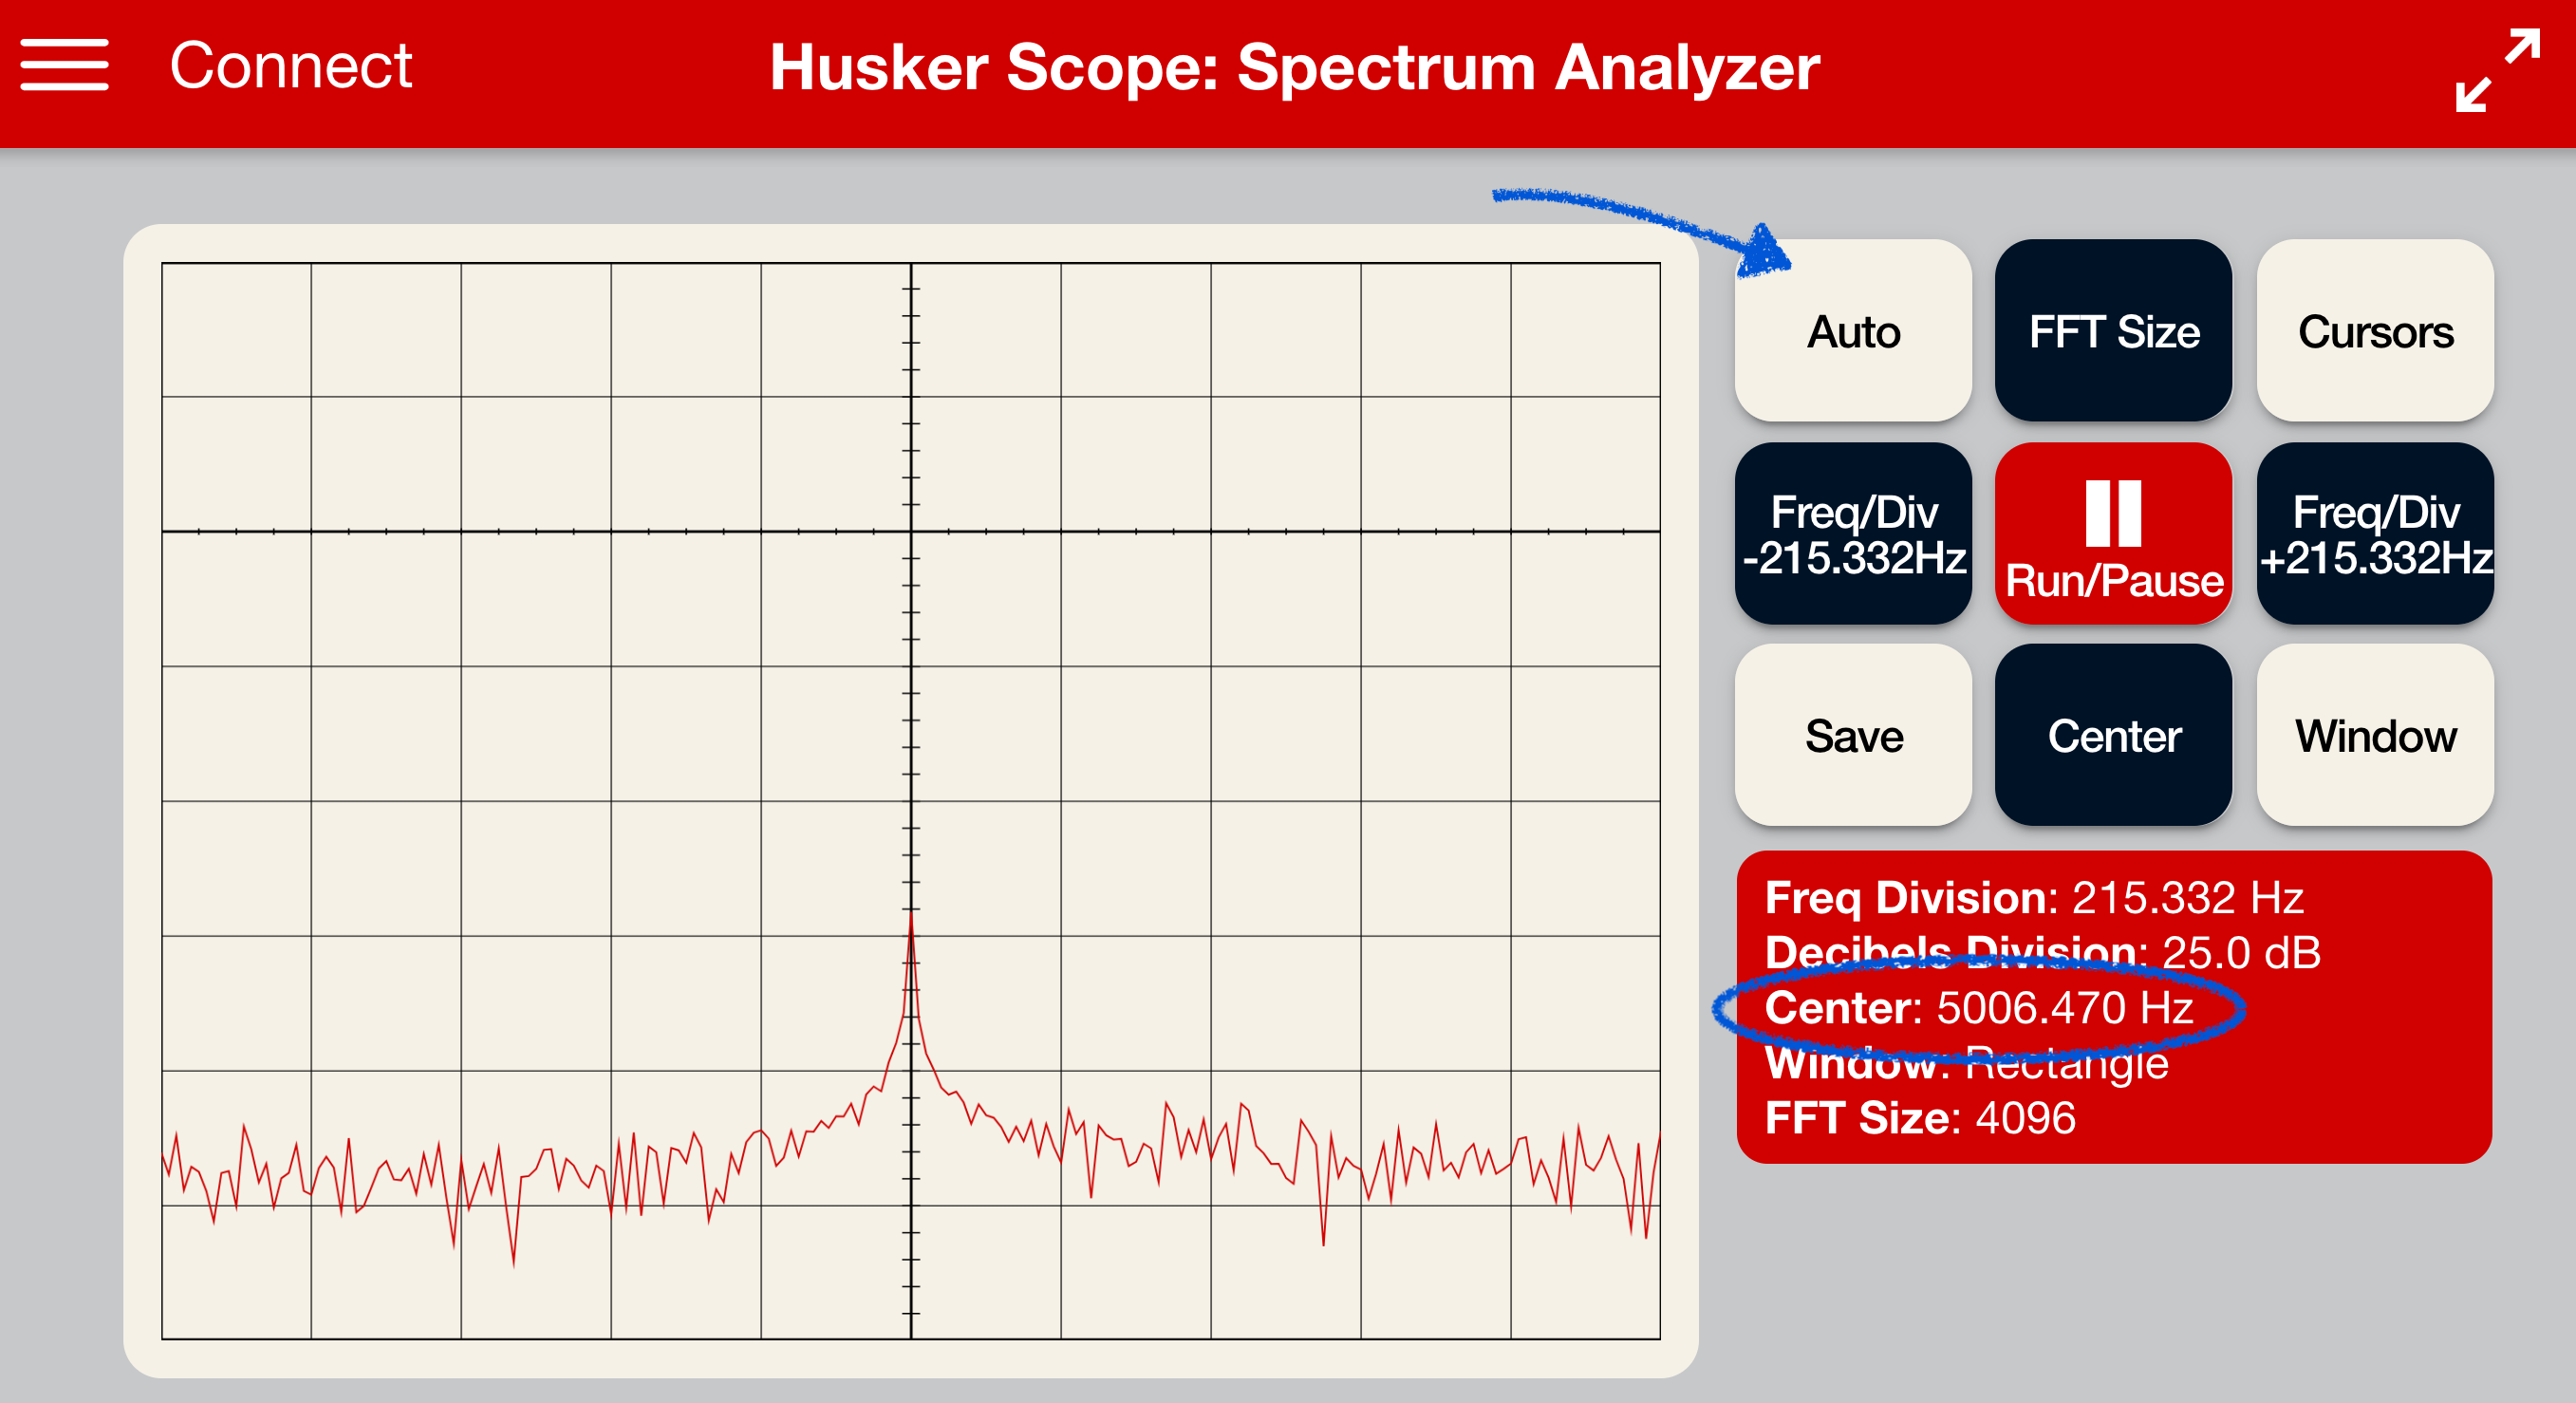
\includegraphics[width=10cm]{SpectrumAnalyzer}
    \caption{Spectrum Analyzer showing a peak near 5kHz \label{fig:spectrumAnalyzer}}
\end{figure}

After your code generates the correct tone, add code so that the continuous tone is generated only when the system is in Continuous Tone mode (Requirements~\ref{spec:modes} \& \ref{spec:continuousTone}).


\subsection{Single-Pulse Operation} \label{subsec:soundSinglePulseOperation}

A fully-correct implementation of Single-Pulse Operation mode has the alarm chirp only if an object is detected closer than the threshold range (Requirement~\ref{spec:singlePulseOperation}).
If you and your partner are working synchronously together -- if you have a working distance sensor -- then temporarily comment-out the code in \function{manage_sensor()} that initiates an ultrasonic pulse.
For the purposes of getting your alarm to chirp, you are temporarily going to have the alarm chirp whenever the pushbutton is pressed.

\vspace{.5cm}

Add another variable that counts the number of times the ISR has been triggered since the start of an alarm.
Add code to increment that counter each time the ISR runs.
You will actually use this variable as a measure of time for the alarm -- if the counter's value is $n$, then there have been $100n$~milliseconds since the start of an alarm.
Since the \lstinline{total_period} variable in the starter code is the amount of time \textit{between} alarms when the system is in Normal Operations mode, add code to reset the counter to 0 when it reaches \lstinline{total_period}. %this, perhaps, belongs in the integration piece

Add another variable that indicates that an alarm should be sounded.

For now, add code that, whenever a ping is requested (see Section~\ref{subsec:readPushbutton}):
\begin{itemize}
    \item The variable indicating that an alarm should be sounded becomes \lstinline{true}
    \item The variable that counts the number of times the ISR has been triggered becomes 0
    \item The variable indicating that a ping is requested becomes \lstinline{false}
\end{itemize}

Recall that the \lstinline{on_period} variable is used to determine how long to generate a tone (and illuminate the LEDs) after detecting an object.
(Since you don't yet have a working distance sensor, you're temporarily choosing to generate a tone whenever the user requests a ping.)
You can now introduce code that will generate the tone whenever these two things are true: an alarm should be sounded, and when the counter is less than \lstinline{on_period}.

Since the piezo should only chirp once, add code to set the ``alarm should be sounded'' variable to \lstinline{false} when the counter exceeds \lstinline{on_period}.

\vspace{.5cm}

Test your code.

\vspace{.5cm}

You may have noticed that when you press the pushbutton, the piezodisc generates a tone for considerably longer than 50ms -- it can hardly be described as a ``chirp.''
Change the value assigned to \lstinline{on_period} to the value that will correctly have the tone generated for only 50ms.

\ifbool{offerdecompositionhints}{
    \paragraph{Hint} What is $50ms \div 100\mu s$?
}{} \\

Now add code to illuminate both LEDs for the same 50ms that the piezodisc generates a tone and then deluminates the LEDs just as the tone is silenced.

\vspace{.5cm}

Most of the object detection work for Single-Pulse Operation takes place in Section~\ref{subsec:distanceSinglePulseOperation}.
You will finish implementing Single-Pulse Operation in Section~\ref{subsec:integrationSpeedSinglePulseOperation} by integrating the detection code from Section~\ref{subsec:distanceSinglePulseOperation} with the alarm code from Section~\ref{subsec:soundSinglePulseOperation}.
This will require small changes to the code.


    \section{Putting it all Together} \label{sec:integration}           The remaining portion of this assignment integrates the work you put into Sections~\ref{sec:initialSoftware}, \ref{sec:distance}, and \ref{sec:sound}.

If you and your partner decided to separately work on Sections~\ref{sec:distance} and \ref{sec:sound}, and if you're still waiting for your partner to finish their section, there is some work in this section that you can get started on.
For example, the user interface portion of Section~\ref{subsubsec:obtainingThreshold} can be while waiting for your partner to finish; however, completing the Threshold Adjustment mode will require the ``distance'' variable from Section~\ref{subsec:distanceSinglePulseOperation}, and making use of the threshold range in Section~\ref{subsubsec:applyingThreshold} requires a working alarm from Section~\ref{subsec:soundSinglePulseOperation}.
Similarly, if you have a working distance sensor, you can do Sections~\ref{subsubsec:repeatedPulses} and \ref{subsubsec:approachRate} without a working alarm, but you will need a working alarm for Section~\ref{subsubsec:repeatedAlarm}.

\subsection{Single-Pulse Operation} \label{subsec:integrationSpeedSinglePulseOperation}

Your distance sensor code responds to a ping request by initiating an ultrasonic pulse, which is what it should do.
Your alarm code responds to a ping request by chirping the piezobuzzer and strobing the right LED;
however, the alarm should only sound if an object has been detected.
There is another incompatibility between the two subsystems:
both set the ping request variable to \lstinline{false} after responding, which means that only one can actually respond to the ping request.

You can resolve this by introducing another shared variable that represents an alarm request.
\begin{description}
    \checkoffitem{When an object is detected, the sensor subsystem should request an alarm.}
    \checkoffitem{When an alarm is requested, the alarm subsystem should chirp the piezobuzzer, strobe the LEDs, and set the alarm request to \lstinline{false} (instead of the ping reqeust).}
\end{description}


\subsection{Threshold Adjustment}

When in Single-Pulse Operation mode, the system now alarms once whenever an object is detected.
Requirement~\ref{spec:singlePulseResponse}, however, says that the LEDs should strobe whenever an object is detected,
but the piezobuzzer should chirp only when the detected object is closer than the threshold range.
\begin{description}
    \checkoffitem{Introduce a shared variable to store the threshold range with an initial value of 400cm, the greatest valid threshold range.}
\end{description}


\subsubsection{Obtaining the Threshold Range} \label{subsubsec:obtainingThreshold}

Requirement~\ref{spec:thresholdAdjustment} describes the user interaction for inputting the threshold range.
Implement this requirement in \textit{user\_controls.c}.

(Note: while you \textit{should} write your code to safely handle a user attempting to enter more than three digits, we will not attempt to do so during grading.)

\begin{description}
    \checkoffitem{After the user has entered a valid threshold range, assign that value to the shared variable.}
\end{description}


\subsubsection{Applying the Threshold Range} \label{subsubsec:applyingThreshold}

You now have the threshold range, externalized from \textit{user\_controls.c}, and the distance to an object, externalized from \textit{sensor.c}.

\begin{description}
    \checkoffitem{Modify the alarm code so that, when in Single-Pulse Operation mode, the alarm strobes the LEDs whenever an object is detected, but it only chirps the piezobuzzer when the distance is no greater than the threshold range.}
\end{description}


\subsection{Normal Operation}

You have now completed every operating mode except ``Normal Operations.''
Look over Requirement~\ref{spec:normalOperation}.

\subsubsection{Repeated Ultrasonic Pulses} \label{subsubsec:repeatedPulses}

When in Normal Operation mode, the sensor does not wait for a ping request.
Instead, it can (and should) send a ping whenever the sensor is in its ``ready'' state.

Modify your code so that:
\begin{description}
    \checkoffitem{When the system is in Normal Operation mode, it initiates a pulse whenever the sensor is ``ready.''}
    \checkoffitem{Re-compute the distance and update the display with each pulse.}
\end{description}

\subsubsection{Compute the Rate of Approach} \label{subsubsec:approachRate}

Since the distance sensor cannot determine the change of direction to the detected object (indeed, it cannot determine the direction), you cannot calculate the object's speed.
You can, however, calculate the longitudinal component of its speed -- that is, how fast it is approaching the sensor.
(A retreating object would, of course, have a negative rate of approach.)
Since the sensor does not detect doppler shift, you must calculate the rate of approach based on the difference between two distance measurements.
There are two options to compute the rate of approach in centimeters per second.
Choose one.
(Or, if you can think of a third approach, you can choose it.)

\begin{description}
    \item[Compare two distances separated in time by 1~second] \phantom{ } \\
        If you have a working alarm subsystem, then you have a timer interrupt firing every 100\textmu s.
        For every 10,000 times that the alarm timer's ISR is triggered, 1~second has passed.
        If you externalize the number of times that the ISR runs, then your code in \textit{sensor.c} can subtract the current distance from the distance calculated 1~second ago.
        The specification does not require that the rate of approach be updated more frequently than once per second, so this is an acceptable approach.
        The only complication is that you'll need to make sure that the user doesn't see an erroneous speed value in the second between obtaining the very first distance after detection and obtaining the second distance.

    \item[Compare the pulse duration for two adjacent measurements] \phantom{ } \\
        Alternatively, you can update the speed every 65,536\textmu s.
        The actual distance travelled will be too small to measure with an integer number of centimeters, so we shall instead rely on the differences in the pulse durations $\tau_1 and \tau_2$.
        Regardless of whether you're using the old hardware or the new hardware, this calculation will need to use 64-bit integers for the intermediate terms.
        If we assume that the wall-clock times of reflection are exactly 65,536\textmu s apart,\footnote{
            If the object is moving, then the actual difference in the wall-clock times of reflection won't be 65,536\textmu s apart; however, the error resulting from this simplifying assumption is less than the rounding error.
        } and that the air temperature does not change appreciably between detections then:
            \begin{description}
                \item[Old Hardware] \phantom{ } \\
                    \begin{align*}
                        speed & = \frac{\Delta distance}{time} %= \frac{\left( \tau_2 \times \frac{18,025 cm}{2^{21}} - \tau_1 \times \frac{18,025 cm}{2^{21}} \right)}{65,536\mu s}
                          = \frac{\left( \tau_2 - \tau_1 \right) \times 18,025 cm}{2^{21} \times 65,536\mu s} \\
                        & \\
                        & =  \left( \tau_2 - \tau_1 \right) \times 281,640,625 \div 2^{31} \ \frac{cm}{s}
                    \end{align*}
                \item[New Hardware] \phantom{ } \\
                    \begin{align*}
                        speed & = \frac{\Delta distance}{time} = \frac{\left( \tau_2 - \tau_1 \right) \times \left( 256,108,888 - 121,907 \times ADC\_register\_value \right) cm}{2^{33} \times 65,536\mu s} \\
                        & \\
                        & =  1,000,000 \times \left( \tau_2 - \tau_1 \right) \times \left( 256,108,888 - 121,907 \times ADC\_register\_value \right) \div 2^{47} \ \frac{cm}{s}
                    \end{align*}
            \end{description}
    \checkoffitem{Add code to \function{manage_sensor()} to calculate the rate of approach when the system is in Normal Operations.}
    \checkoffitem{Whenever you have calculated a new rate of approach, update the display with that rate of approach.}
\end{description}

\subsubsection{Repeated Alarm} \label{subsubsec:repeatedAlarm}

Your remaining task is to repeatedly activate the alarm when in Normal Operations.
You probably noticed the \lstinline{total_period} variable in \textit{alarm.c}, immediately below the \lstinline{on_period} variable.
Just as \lstinline{on_period} is used to determine how long the piezobuzzer should emit its tone and the LEDs should be illuminated, the \lstinline{total_period} is used to determine how much time should transpire between activations of the alarm.
(If you wish, you can imagine a \lstinline{off_period} variable whose value is always \lstinline{total_period} - \lstinline{on_period}.)

\paragraph{Repeatedly activate the alarm}
\begin{description}
    \checkoffitem{Add code so that, when an object is detected while the system is in Normal Operations mode, the alarm will repeatedly activate.}
        \begin{itemize}
            \item We recommend that you use the \lstinline{total_period} variable as part of that solution.
        \end{itemize}
\end{description}
\paragraph{Vary the time between activations}
\begin{description}
    \checkoffitem{Using Table~\ref{tab:alarmPeriods} and the distance to the detected object, change \lstinline{total_period}'s value so that the time between alarm activations is correct.}
\end{description}


    \section{Turn-in and Grading}                                       \filesubmission.

\policyforcodethatdoesnotcompile

\latepolicy

\subsection*{Rubric}

This assignment is worth 35 points.
\begin{description}
    \rubricitem{1}{\function{is_nan()} correctly reports whether or not its argument is a number}
    \rubricitem{1}{\function{is_zero()} correctly reports whether or not its argument is zero}
    \rubricitem{1}{\function{is_infinity()} correctly reports whether or not its argument is infinite}
    \rubricitem{1}{\function{is_negative()} correctly reports whether or not its argument is negative}
    \rubricitem{1}{\function{get_754_integer()} correctly extracts the significand's implicit integer}
    \rubricitem{1}{\function{get_754_fraction()} correctly extracts the significand's fraction bits}
    \rubricitem{1}{\function{get_754_exponent()} correctly extracts the exponent}
    \rubricitem{1}{\function{decode()} correctly converts an \lstinline{ieee754_t} value into a \lstinline{unnormal_t} structure}
    \rubricitem{1}{\function{negate()} correctly changes its argument's sign}
    \rubricitem{5}{\function{add()} can add integers \& fractions, positive \& negative values, and ``large'' \& ``small'' numbers}
    \rubricitem{1}{The identity and commutative properties hold for \function{add()}}
    \rubricitem{1}{\function{add()} provides correct answers for its special cases}
    \rubricitem{5}{\function{multiply()} can multiply integers \& fractions, positive \& negative values, and ``large'' \& ``small'' numbers}
    \rubricitem{2}{The identity, zero, and commutative properties hold for \function{multiply()}}
    \rubricitem{1}{\function{multiply()} provides correct answers for its special cases}
    \rubricitem{1}{\function{divide()} provides correct answers for its special cases}
    \rubricitem{1}{\function{divide()} can divide when the divisor is of the form $\pm 2^n, -126 \le n \le 127$}
    \rubricitem{1}{\function{divide()} can divide when the dividend's significand is a multiple of the divisor's significand}
    \rubricitem{1}{\function{add()} demonstrates that \function{encode()} rounds down when the truncated part of the significand is less than halfway between representable values}
    \rubricitem{1}{\function{add()} demonstrates that \function{encode()} rounds up when the truncated part of the significand is more than halfway between representable values}
    \rubricitem{2}{\function{add()} demonstrates that \function{encode()} rounds to the nearest-even when the truncated part of the significand is exactly halfway between representable values}
    \rubricitem{1}{Rounding can carry into the exponent}
    \rubricitem{1}{\function{add()} and/or \function{multiply()} demonstrate that \function{encode()} overflows to infinity}
    \rubricitem{1}{\function{add()}, \function{multiply()}, and/or \function{divide()} demonstrate that \function{encode()} gracefully underflows through subnormal numbers}
    \rubricitem{1}{\function{multiply()} and/or \function{divide()} demonstrate that \function{encode() underflows to zero}}
    \bonusitem{2}{\function{divide()} can divide arbitrary values}
\end{description}

\textbf{Penalties}
\begin{description}
    \softwareengineeringpenalties
    \item[no credit] for functions that use \lstinline{float} or \lstinline{double} variables or constants, use \lstinline{union} variables, use C's floating point operations, and/or a function you did not write
    \item[no credit] for arithmetic functions, if \function{decode()} and/or \function{encode()}  use \lstinline{float} or \lstinline{double} variables or constants, use \lstinline{union} variables, use C's floating point operations, and/or a function you did not write
\end{description}


    \section*{Epilogue}                                                 \RangeFinderDetecting

    \textit{The end...?}

%    \newpage\appendix
    \appendix

    \section{Appendix: Lab Checkoff}                                    You are not required to have your assignment checked-off by a TA or the professor.
If you do not do so, then we will perform a functional check ourselves.
In the interest of making grading go faster, we are offering a small bonus to get your assignment checked-off at the start of your scheduled lab time immediately after it is due.
Because checking off all students during lab would take up most of the lab time, we are offering a slightly larger bonus if you complete your assignment early and get it checked-off by a TA or the professor during office hours.

\begin{enumerate}
    \precheckoffitem{Position the Cow Pi a little more than 1~meter from a wall, or position an upright book (or other object) a little more than 1~meter from the Cow Pi.}
    \precheckoffitem{Place both switches in the left position.}
    \precheckoffitem{Upload your code to your \developmentboard, and leave your code open in the IDE.}
    \precheckoffitem{Confirm that the system detects the wall (or book or other object) and not something closer (such as a computer or the table surface).}

    \checkoffitem{Show and explain to the TA how your code generates a tone with a frequency of 5kHz; that is, it has a period of 200\textmu s.}
    \checkoffitem{Place the right switch in the right position, putting the system in Continuous Tone mode.
        The system generates a continuous 5kHz tone.}
    \item[] (TA, confirm that the tone is 5kHz by code inspection and by ear; confirm with the HuskerScope spectrum analyzer if you aren't sure.) \\
        \textit{+1 There is code to generate an audible tone} \\
        \textit{+1 The system continuously generates the tone when in Continuous Tone mode} \\
        \textit{+2 The audible tone has a frequency of 5kHz}

    \checkoffitem{Place the left switch in the right position, putting the system in Threshold Adjustment mode.
        The system prompts for a new threshold range. \\
        \textit{+1 The user is prompted to enter a new threshold range when the system is in Threshold Adjustment mode}}
    \checkoffitem{Enter a range of 25, using the `\#' key to indidicate that you have fininished entering the value.
        The system displays a helpful error message explaining that this is not a valid threshold range.
        The system then prompts the user for a new threshold range. \\
        \textit{+1 The user is given a helpful error message after entering an invalid threshold range} \\
        \textit{+1 The user is re-prompted to enter a threshold range after entering an invalid threshold range}}
    \checkoffitem{Enter a range of 450, using the `\#' key to indidicate that you have fininished entering the value.
        The system displays a helpful error message explaining that this is not a valid threshold range.
        The system then prompts the user for a new threshold range.}
    \checkoffitem{Enter a range of 75, using the `\#' key to indidicate that you have fininished entering the value.
        The system displays a message confirming the new threshold range. \\
        \textit{+2 Valid threshold ranges are those between 50cm and 400cm, inclusive} \\
        \textit{+1 The user is shown a confirmation message after entering a valid threshold range} \\
        \textit{+2 The user can enter a new threshold range when the system is in Threshold Adjustment mode}}

    \checkoffitem{Place the right switch in the left position, putting the system in Single Pulse mode.
        The system might indicate that no object has been detected yet; however, this is not required information before initiating a ping.}
    \checkoffitem{Show and explain to the TA how your code initiates a pulse.}
    \checkoffitem{Show and explain to the TA how your code measures the length of a pulse.}
    \checkoffitem{Show and explain to the TA how your code achieves the required precision (no greater than 1\textmu s) and accuracy (immediately detect pulse edges without waiting for code in the main loop to poll the pin).}
    \checkoffitem{Press the pushbutton to initiate a pulse.
        The right LED strobes once.
        The piezodisc does not chirp.
        The system displays the correct distance to the wall (or book or other object). \\
        \textit{+2 There is code to initiate an ultrasound pulse} \\
        \textit{+3 There is code to detect the length of the pulse} \\
        \textit{+3 The pulse's length is measured to a precision of no greater than 1\textmu s} \\
        \textit{+3 The pulse's length is measured as accurately as possible} \\
        \textit{+2 The user can request a ping when the system is in Single Pulse mode} \\
        \textit{+2 The distance to an object is correctly calculated from the pulse's length} \\
        \textit{+2 When an object is detected, the system displays the distance to the object} \\
        \textit{+2 When an object is detected in Single-Pulse mode, the system generates exactly one alarm} \\
        \textit{+2 A strobe is an illumination of the right LED for 50ms} \\
        \textit{+2 A strobe occurs for any detected object}}
    \checkoffitem{Slightly change the distance between the Cow Pi and the target object.
        Press the pushbutton to initiate a pulse.
        The LED strobes once.
        The piezodisc does not chirp.
        The system displays the new distance to the wall (or book or other object). \\
        \textit{+2 The user can request another ping when the system is in Single Pulse mode}}

    \checkoffitem{Place the left switch in the left position, putting the system in Normal Operation mode.
        The system displays the distance to the target object, and it displays an approach rate of 0cm/s.
        The LED strobes once per seccond (100ms), but the piezodisc does not chirp. \\
        \textit{+1 The switches control the mode of operation as specified} \\
        \textit{+2 When an object is detected in Normal Operation mode, the system repeatedly generates alarms}}
    \checkoffitem{Slowly move the Cow Pi closer to the wall, or slowly move the book (or other object) closer to the Cow Pi.
        As you do so, vary the rate of approach slighly to demonstrate that the rate of approach updates.
        The displayed distance changes with the decreasing distance to the target object.
        The system displays a plausible, positive rate of approach that updates at least once every second. \\
        \textit{+2 When an object is detected in Normal Operation mode the rate of approach is displayed} \\
        \textit{+2 When an object is detected in Normal Operation mode, the rate of approach is updated at least once every second}}
    \checkoffitem{As the distance between the Cow Pi and the target object decreases, note that:
        \begin{description}
            \item[When the distance falls below 100cm] the LED strobes more frequently, once every 750ms (\textthreequarters sec)
            \item[When the distance falls below 75cm] the piezodisc chirps every 750ms
            \item[When the distance falls below 50cm] the LED strobes, and the piezodisc chirps, every 500ms (\textonehalf sec)
            \item[When the distance falls below 25cm] the LED strobes, and the piezodisc chirps, every 250ms (\textonequarter sec)
            \item[When the distance falls below 10cm] the LED strobes, and the piezodisc chirps, every 125ms ($\frac{1}{8}$ sec)
        \end{description}
        \textit{+2 A chirp is an audible tone lasting 50ms} \\
        \textit{+2 When the system repeatedly generates alarms, the time between alarms is as specified}}

    \checkoffitem{Place the both switches in the right position, putting the system in Threshold Adjustment mode.
        The system prompts for a new threshold range.}
    \checkoffitem{Enter a range of 55.
        The system displays a message confirming the new threshold range.}
    \checkoffitem{Place the both switches in the left position, putting the system in Normal Operation mode.
        The system displays the distance to the target object, and it displays an approach rate of 0cm/s.}
    \checkoffitem{Slowly move the Cow Pi away from the wall, or slowly move the book (or other object) away from the Cow Pi.
        The displayed distance changes with the decreasing distance to the target object.
        The system displays a plausible, negative rate of approach.}
    \checkoffitem{As the distance between the Cow Pi and the target object decreases, the alarms become less urgent.
        Note that as the distance increases above 55cm, the piezodisc stops chirping but the LED continues to strobe. \\
        \textit{+2 A chirp occurs for a detected object that is closer than the threshold range} \\
        \textit{+2 A chirp only occurs for a detected object that is closer than the threshold range}}

    \checkoffitem{Reorient the Cow Pi, or remove the book (or other object) so that there are no in-range objects to detect.
        The system displays a message indicating that no object is detected.
        The LED does not strobe, and the piezodisc does not chirp.\\
        \textit{+3 The code correctly recognizes the that no object has been detected, if no object reflects the ultrasound pulse} \\
        \textit{+2 When there is no in-range object, the system displays a message to that effect} \\
        \textit{+2 A strobe only occurs for a detected object}}

    \checkoffitem{Show the TA any code they have not yet examined. \\
        \textit{+1 The code is clean, well-organized, has good variable and function names, and is otherwise understandable}}
\end{enumerate}

    \section{Appendix: Handling Phantom Interrupts} \label{sec:phantom} Some students have encountered what might be called ``phantom interrupts'' when the system initially powers-up.
If your system is in Single Pulse mode when initially powered up, this could cause what appears to be an object detection despite not having pressed the button.
We'reno aware of this issue, and our plan during grading is to politely ignore it when that happens immediately upon starting the program.

If it bugs you enough, you can address it through the sensor’s state machine.

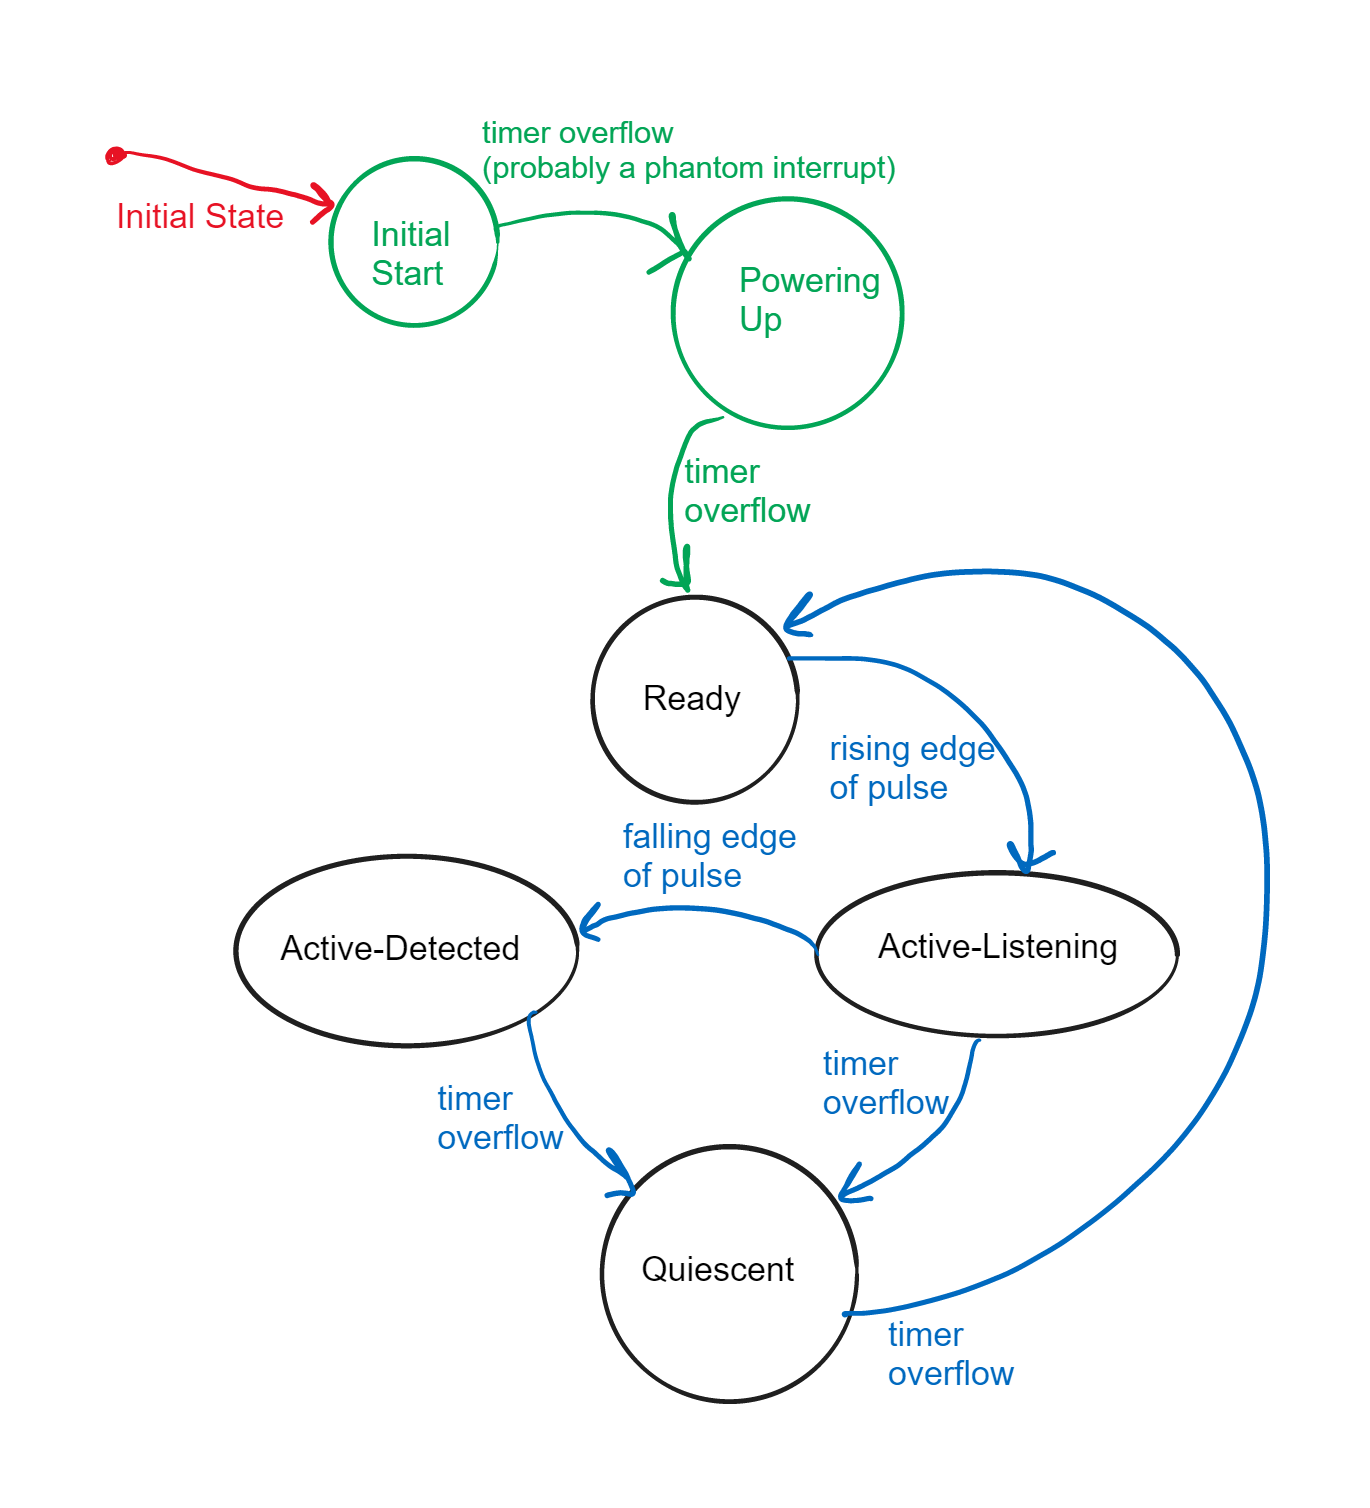
\includegraphics[width=4in]{noPhantomInterrupts}

Nothing happens in the ``Initial Start'' and ``Powering Up'' states – in fact, that’s the point of them.
If you only respond to pulse edges when you’re in the ``Ready'' state or the ``Active-Listening'' state, then phantom pin change interrupts that happen when powering-up the system won’t affect anything.
They’ll happen in the first few dozen nanoseconds, when your system is either in the ``Initial Start'' state or the ``Powering Up'' state.
(We don’t know whether the phantom pin change interrupt, if it happens, will occur before or after the phantom timer interrupt, if it occurs, which is why we have two do-nothing states.)

\end{document}
